\chapter{Heap di Fibonacci}\label{ch:heap-fibonacci}
Gli \textbf{heap di Fibonacci} sono la seconda implementazione dei mergeable heap che studiamo, dopo gli heap binomiali del capitolo~\ref{ch:heap-binomiali}. Supportano le stesse operazioni, ma con costi ammortizzati migliori: l'inserimento, l'unione e il decremento di una chiave costano $O(1)$, mentre l'estrazione del minimo e la cancellazione costano $O(\lg n)$. Sono stati introdotti da M.\,L.~Fredman e R.\,E.~Tarjan tra il 1984 e il 1987.

Come un heap binomiale, un heap di Fibonacci è una collezione di alberi con la proprietà di min-heap. Cambia però il modo in cui la collezione viene mantenuta. Un heap binomiale riorganizza i suoi alberi a ogni operazione, mentre un heap di Fibonacci rimanda questo lavoro il più a lungo possibile, e lo svolge tutto insieme durante l'estrazione del minimo. Per questo motivo, i costi si studiano con l'analisi ammortizzata, e in particolare con il metodo del potenziale (sezione~\ref{sec:potenziale}).

Il nome viene dai numeri di Fibonacci, che compaiono nella dimostrazione del limite al grado dei nodi, alla fine del capitolo.

\section{Struttura}\label{sec:hf-struttura}
A differenza di un heap binomiale, un heap di Fibonacci non impone ai suoi alberi una forma precisa.

\begin{definizione}[Heap di Fibonacci]\label{def:heap-fibonacci}
Un \textbf{heap di Fibonacci} $H$ è una collezione di alberi radicati, ciascuno dei quali gode della proprietà di \textbf{min-heap}: la chiave di ogni nodo è maggiore o uguale alla chiave di suo padre.
\end{definizione}

Gli alberi di un heap di Fibonacci, quindi, non devono essere alberi binomiali. Non si tratta però di alberi qualsiasi: vedremo che sono alberi binomiali non ordinati, eventualmente ``erosi'' dai tagli che esegue il decremento di una chiave.

Con $D(n)$ indichiamo il \textbf{grado massimo} di un nodo in un heap di Fibonacci con $n$ nodi, dove il grado di un nodo è il numero dei suoi figli.

\paragraph{Costi.}
La tabella~\ref{tab:hb-confronto} confronta i costi degli heap di Fibonacci con quelli degli heap binari e binomiali. Per gli heap di Fibonacci si tratta di costi ammortizzati. In particolare, l'estrazione del minimo e la cancellazione costano $O(D(n))$.

Senza altre informazioni sappiamo soltanto che $D(n) \le n - 1$, il grado di una radice che ha come figli tutti gli altri nodi. Dimostreremo che in realtà:
\[
D(n) \le \lfloor \log_\phi n \rfloor = O(\lg n),
\]
dove $\phi = (1+\sqrt{5})/2 \approx 1{,}618$ è il \textbf{rapporto aureo} (o sezione aurea). Ne segue il costo $O(\lg n)$ riportato in tabella.

\subsection{Rappresentazione}\label{sec:hf-rappresentazione}
Ogni nodo $x$ di un heap di Fibonacci ha i seguenti campi (figura~\ref{fig:hf-nodo}):
\begin{itemize}
    \item $\mathit{key}[x]$: la chiave, insieme alle eventuali informazioni satellite.
    \item $p[x]$: un puntatore al padre, che vale \Nil{} se $x$ è una radice.
    \item $\mathit{left}[x]$ e $\mathit{right}[x]$: i puntatori al fratello sinistro e al fratello destro.
    \item $\mathit{child}[x]$: un puntatore a uno qualsiasi dei figli, che vale \Nil{} se $x$ non ha figli.
    \item $\mathit{degree}[x]$: il grado di $x$, ovvero il numero dei suoi figli.
    \item $\mathit{mark}[x]$: un valore booleano che indica se $x$ ha perso un figlio dall'ultima volta in cui è diventato figlio di un altro nodo.
\end{itemize}

\begin{figure}[htbp]
\centering
\begin{tikzpicture}[binheap, >=Stealth]
  \draw[Accent, fill=Accent!6] (-1.35,0.72) rectangle (1.35,-0.72);
  \draw[Accent] (-1.35,0.24) -- (1.35,0.24);
  \draw[Accent] (-1.35,-0.24) -- (1.35,-0.24);
  \draw[Accent] (-0.45,0.72) -- (-0.45,0.24);
  \draw[Accent] (0,0.24) -- (0,-0.24);
  \draw[Accent] (-0.45,-0.24) -- (-0.45,-0.72);
  \draw[Accent] (0.45,-0.24) -- (0.45,-0.72);
  \node[font=\small] at (-0.9,0.48) {$p$};
  \node[font=\small] at (0.45,0.48) {$\mathit{key}$};
  \node[font=\small] at (-0.675,0) {$\mathit{degree}$};
  \node[font=\small] at (0.675,0) {$\mathit{mark}$};
  \node[font=\small] at (-0.9,-0.48) {$\mathit{left}$};
  \node[font=\small] at (0,-0.48) {$\mathit{child}$};
  \node[font=\small] at (0.9,-0.48) {$\mathit{right}$};
  \draw[->, ptrp] (-0.9,0.72) -- (-0.9,1.25) node[lab, right] {padre};
  \draw[->, ptrs] (-1.35,-0.48) -- (-1.95,-0.48) node[lab, left] {fratello sinistro};
  \draw[->, ptrs] (1.35,-0.48) -- (1.95,-0.48) node[lab, right] {fratello destro};
  \draw[->, ptrc] (0,-0.72) -- (0,-1.25) node[lab, below] {uno dei figli};
\end{tikzpicture}
\caption{I campi di un nodo $x$ di un heap di Fibonacci. Oltre alla chiave, il nodo ha un puntatore al padre, ai due fratelli e a uno qualsiasi dei figli, il grado e il bit $\mathit{mark}[x]$.}
\label{fig:hf-nodo}
\end{figure}

I figli di un nodo formano una \textbf{lista circolare doppiamente concatenata}, tramite i campi $\mathit{left}$ e $\mathit{right}$. Se $x$ è figlio unico, si ha $\mathit{left}[x] = \mathit{right}[x] = x$. L'ordine dei figli nella lista è arbitrario. Le liste circolari doppiamente concatenate hanno due vantaggi, che useremo spesso:
\begin{itemize}
    \item Un nodo si inserisce o si toglie in qualsiasi punto della lista in tempo $O(1)$.
    \item Due liste si concatenano in un'unica lista circolare in tempo $O(1)$.
\end{itemize}

Partendo da un nodo qualsiasi, la lista si può percorrere in due versi, seguendo i campi $\mathit{right}$ oppure i campi $\mathit{left}$. In pratica, è come scegliere tra la circolare destra e la circolare sinistra (figura~\ref{fig:hf-circolari}).

\begin{figure}[htbp]
\centering
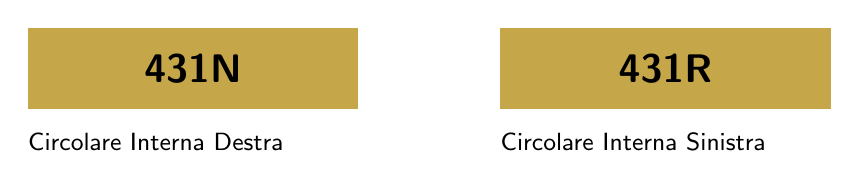
\begin{tikzpicture}[font=\sffamily]
  \definecolor{circolare}{HTML}{C5A648}
  \foreach \x/\linea/\verso in {0/431N/Destra, 6/431R/Sinistra} {
    \fill[circolare] (\x,0) rectangle ++(4.2,1.03);
    \node[font=\sffamily\bfseries\Large] at (\x+2.1,0.515) {\linea};
    \node[anchor=north west, inner sep=0pt, font=\small\sffamily\fontseries{sb}\selectfont] at (\x,-0.3) {Circolare Interna \verso};
  }
\end{tikzpicture}
\caption{La versione catanese di una lista circolare doppiamente concatenata: la 431N segue i puntatori $\mathit{right}$, la 431R i puntatori $\mathit{left}$. In entrambi i casi, prima o poi, si torna alla fermata di partenza. Su quel ``prima o poi'', però, nessuno ha ancora dimostrato un limite superiore.}
\label{fig:hf-circolari}
\end{figure}

Anche le radici degli alberi sono collegate tramite i campi $\mathit{left}$ e $\mathit{right}$, e formano la \textbf{lista delle radici}, circolare e doppiamente concatenata, in cui gli alberi possono comparire in qualsiasi ordine. L'heap è individuato da un puntatore $\mathit{min}[H]$ alla radice con la chiave minima, che è il punto di accesso alla struttura e vale \Nil{} se l'heap è vuoto. Infine $n[H]$ è il numero di nodi di $H$.\footnote{Per i campi di un oggetto si trova anche la notazione con il punto: $H.\mathit{min}$ indica lo stesso campo di $\mathit{min}[H]$.}

La figura~\ref{fig:hf-esempio} mostra un heap di Fibonacci con $14$ nodi e cinque alberi, prima nella forma che useremo nei disegni e poi con tutti i puntatori. I nodi marcati sono disegnati in nero.

\begin{figure}[htbp]
\centering
%% GEN:esempio
\begin{tikzpicture}[fibheap, >=Stealth]
  % (a)
  \node[lab, anchor=east] at (0.500,-0.750) {(a)};
  \node[hn] (e0n0) at (0.814,-0.750) {23};
  \node[hn] (e0n1) at (1.525,-0.750) {7};
  \node[hm] (e0n4) at (2.236,-1.947) {39};
  \node[hm] (e0n3) at (2.236,-1.348) {18};
  \node[hn] (e0n5) at (2.763,-1.348) {52};
  \node[hn] (e0n7) at (3.290,-1.947) {41};
  \node[hn] (e0n6) at (3.290,-1.348) {38};
  \node[hn] (e0n2) at (2.763,-0.750) {3};
  \node[hn] (e0n9) at (4.002,-1.348) {30};
  \node[hn] (e0n8) at (4.002,-0.750) {17};
  \node[hn] (e0n12) at (4.713,-1.947) {35};
  \node[hm] (e0n11) at (4.713,-1.348) {26};
  \node[hn] (e0n13) at (5.240,-1.348) {46};
  \node[hn] (e0n10) at (4.977,-0.750) {24};
  \draw (e0n2) -- (e0n3);
  \draw (e0n3) -- (e0n4);
  \draw (e0n2) -- (e0n5);
  \draw (e0n2) -- (e0n6);
  \draw (e0n6) -- (e0n7);
  \draw (e0n8) -- (e0n9);
  \draw (e0n10) -- (e0n11);
  \draw (e0n11) -- (e0n12);
  \draw (e0n10) -- (e0n13);
  \draw[rl] (e0n0) -- (e0n1);
  \draw[rl] (e0n1) -- (e0n2);
  \draw[rl] (e0n2) -- (e0n8);
  \draw[rl] (e0n8) -- (e0n10);
  \node[head, anchor=south] (e0min) at (2.763,-0.330) {$\mathit{min}[H]$};
  \draw[->] (e0min) -- (e0n2);
\end{tikzpicture}
%% END:esempio

\vspace{5mm}
%% GEN:rappresentazione
\begin{tikzpicture}[fibheap, >=Stealth]
  \node[lab, anchor=east] at (-0.1,0) {(b)};
  \node[hn] (rn0) at (0.810,0.000) {23};
  \node[hn] (rn1) at (2.391,0.000) {7};
  \node[hm] (rn4) at (3.972,-2.640) {39};
  \node[hm] (rn3) at (3.972,-1.320) {18};
  \node[hn] (rn5) at (4.992,-1.320) {52};
  \node[hn] (rn7) at (6.012,-2.640) {41};
  \node[hn] (rn6) at (6.012,-1.320) {38};
  \node[hn] (rn2) at (4.992,0.000) {3};
  \node[hn] (rn9) at (7.593,-1.320) {30};
  \node[hn] (rn8) at (7.593,0.000) {17};
  \node[hn] (rn12) at (9.174,-2.640) {35};
  \node[hm] (rn11) at (9.174,-1.320) {26};
  \node[hn] (rn13) at (10.194,-1.320) {46};
  \node[hn] (rn10) at (9.684,0.000) {24};
  \draw[->, ptrs] ([yshift=1.3pt]rn0.east) -- ([yshift=1.3pt]rn1.west);
  \draw[->, ptrs] ([yshift=-1.3pt]rn1.west) -- ([yshift=-1.3pt]rn0.east);
  \draw[->, ptrs] ([yshift=1.3pt]rn1.east) -- ([yshift=1.3pt]rn2.west);
  \draw[->, ptrs] ([yshift=-1.3pt]rn2.west) -- ([yshift=-1.3pt]rn1.east);
  \draw[->, ptrs] ([yshift=1.3pt]rn2.east) -- ([yshift=1.3pt]rn8.west);
  \draw[->, ptrs] ([yshift=-1.3pt]rn8.west) -- ([yshift=-1.3pt]rn2.east);
  \draw[->, ptrs] ([yshift=1.3pt]rn8.east) -- ([yshift=1.3pt]rn10.west);
  \draw[->, ptrs] ([yshift=-1.3pt]rn10.west) -- ([yshift=-1.3pt]rn8.east);
  \draw[->, ptrs, rounded corners=1.5pt] ([yshift=1.3pt]rn10.east) -- ++(0.13,0) |- ($(rn0.west)+(-0.13,0.3)$) |- ([yshift=1.3pt]rn0.west);
  \draw[->, ptrs, rounded corners=1.5pt] ([yshift=-1.3pt]rn0.west) -- ++(-0.13,0) |- ($(rn10.east)+(0.13,-0.3)$) |- ([yshift=-1.3pt]rn10.east);
  \draw[->, ptrs] ([yshift=1.3pt]rn3.east) -- ([yshift=1.3pt]rn5.west);
  \draw[->, ptrs] ([yshift=-1.3pt]rn5.west) -- ([yshift=-1.3pt]rn3.east);
  \draw[->, ptrs] ([yshift=1.3pt]rn5.east) -- ([yshift=1.3pt]rn6.west);
  \draw[->, ptrs] ([yshift=-1.3pt]rn6.west) -- ([yshift=-1.3pt]rn5.east);
  \draw[->, ptrs, rounded corners=1.5pt] ([yshift=1.3pt]rn6.east) -- ++(0.13,0) |- ($(rn3.west)+(-0.13,0.3)$) |- ([yshift=1.3pt]rn3.west);
  \draw[->, ptrs, rounded corners=1.5pt] ([yshift=-1.3pt]rn3.west) -- ++(-0.13,0) |- ($(rn6.east)+(0.13,-0.3)$) |- ([yshift=-1.3pt]rn6.east);
  \draw[->, ptrc] (rn2) to[bend left=12] (rn3);
  \draw[->, ptrp] (rn3) to[bend left=12] (rn2);
  \draw[->, ptrp] (rn5) -- (rn2);
  \draw[->, ptrp] (rn6) -- (rn2);
  \draw[->, ptrs, rounded corners=1.5pt] ([yshift=1.3pt]rn4.east) -- ++(0.13,0) |- ($(rn4.west)+(-0.13,0.3)$) |- ([yshift=1.3pt]rn4.west);
  \draw[->, ptrs, rounded corners=1.5pt] ([yshift=-1.3pt]rn4.west) -- ++(-0.13,0) |- ($(rn4.east)+(0.13,-0.3)$) |- ([yshift=-1.3pt]rn4.east);
  \draw[->, ptrc] (rn3) to[bend left=12] (rn4);
  \draw[->, ptrp] (rn4) to[bend left=12] (rn3);
  \draw[->, ptrs, rounded corners=1.5pt] ([yshift=1.3pt]rn7.east) -- ++(0.13,0) |- ($(rn7.west)+(-0.13,0.3)$) |- ([yshift=1.3pt]rn7.west);
  \draw[->, ptrs, rounded corners=1.5pt] ([yshift=-1.3pt]rn7.west) -- ++(-0.13,0) |- ($(rn7.east)+(0.13,-0.3)$) |- ([yshift=-1.3pt]rn7.east);
  \draw[->, ptrc] (rn6) to[bend left=12] (rn7);
  \draw[->, ptrp] (rn7) to[bend left=12] (rn6);
  \draw[->, ptrs, rounded corners=1.5pt] ([yshift=1.3pt]rn9.east) -- ++(0.13,0) |- ($(rn9.west)+(-0.13,0.3)$) |- ([yshift=1.3pt]rn9.west);
  \draw[->, ptrs, rounded corners=1.5pt] ([yshift=-1.3pt]rn9.west) -- ++(-0.13,0) |- ($(rn9.east)+(0.13,-0.3)$) |- ([yshift=-1.3pt]rn9.east);
  \draw[->, ptrc] (rn8) to[bend left=12] (rn9);
  \draw[->, ptrp] (rn9) to[bend left=12] (rn8);
  \draw[->, ptrs] ([yshift=1.3pt]rn11.east) -- ([yshift=1.3pt]rn13.west);
  \draw[->, ptrs] ([yshift=-1.3pt]rn13.west) -- ([yshift=-1.3pt]rn11.east);
  \draw[->, ptrs, rounded corners=1.5pt] ([yshift=1.3pt]rn13.east) -- ++(0.13,0) |- ($(rn11.west)+(-0.13,0.3)$) |- ([yshift=1.3pt]rn11.west);
  \draw[->, ptrs, rounded corners=1.5pt] ([yshift=-1.3pt]rn11.west) -- ++(-0.13,0) |- ($(rn13.east)+(0.13,-0.3)$) |- ([yshift=-1.3pt]rn13.east);
  \draw[->, ptrc] (rn10) to[bend left=12] (rn11);
  \draw[->, ptrp] (rn11) to[bend left=12] (rn10);
  \draw[->, ptrp] (rn13) -- (rn10);
  \draw[->, ptrs, rounded corners=1.5pt] ([yshift=1.3pt]rn12.east) -- ++(0.13,0) |- ($(rn12.west)+(-0.13,0.3)$) |- ([yshift=1.3pt]rn12.west);
  \draw[->, ptrs, rounded corners=1.5pt] ([yshift=-1.3pt]rn12.west) -- ++(-0.13,0) |- ($(rn12.east)+(0.13,-0.3)$) |- ([yshift=-1.3pt]rn12.east);
  \draw[->, ptrc] (rn11) to[bend left=12] (rn12);
  \draw[->, ptrp] (rn12) to[bend left=12] (rn11);
  \node[head, anchor=south] (rmin) at (4.992,0.700) {$\mathit{min}[H]$};
  \draw[->] (rmin) -- ([yshift=0.32cm]rn2.north) -- (rn2);
\end{tikzpicture}
%% END:rappresentazione
\caption{(a) Un heap di Fibonacci con $14$ nodi e cinque alberi. Le linee tratteggiate collegano le radici nella lista delle radici, e $\mathit{min}[H]$ punta alla radice con la chiave minima. I nodi $18$, $39$ e $26$ sono marcati, e sono disegnati in nero. (b) Lo stesso heap con tutti i puntatori: le liste dei fratelli e la lista delle radici sono circolari e doppiamente concatenate (in verde scuro), ogni padre punta a uno dei figli (in viola) e ogni figlio punta al padre (in grigio).}
\label{fig:hf-esempio}
\end{figure}

\section{Funzione potenziale}\label{sec:hf-potenziale}
I costi delle operazioni si studiano con il metodo del potenziale. Per un heap di Fibonacci $H$ si definisce la \textbf{funzione potenziale}:
\[
\Phi(H) = t(H) + 2\, m(H),
\]
dove $t(H)$ è il numero di alberi nella lista delle radici di $H$, e $m(H)$ è il numero di nodi marcati in $H$. Ad esempio, l'heap della figura~\ref{fig:hf-esempio} ha cinque alberi e tre nodi marcati, quindi $\Phi(H) = 5 + 2 \cdot 3 = 11$.

Un'applicazione lavora in genere con più heap. Per una collezione finita $\{H_i\}_{i \in I}$ di heap di Fibonacci poniamo:
\[
\Phi\bigl(\{H_i\}_{i \in I}\bigr) = \sum_{i \in I} \Phi(H_i) \ge 0 = \Phi(\emptyset),
\]
dove $\emptyset$ indica la collezione vuota di heap di Fibonacci. Il potenziale parte quindi da $0$ e non è mai negativo, e la somma dei costi ammortizzati è un limite superiore alla somma dei costi effettivi.

Supponiamo inoltre che un'unità di potenziale basti a pagare una qualsiasi delle operazioni di costo costante che incontreremo. Se necessario, si moltiplica il potenziale per una costante opportuna. Il motivo del coefficiente $2$ davanti a $m(H)$ sarà chiaro con il decremento di una chiave.

\paragraph{Il grado massimo.}
L'analisi è espressa in funzione di $D(n)$, il limite superiore al grado massimo di un nodo qualunque in un heap di Fibonacci con $n$ nodi. Fino alla sezione~\ref{sec:hf-grado} lo useremo come un parametro, e solo alla fine dimostreremo che $D(n) = O(\lg n)$.

\section{Alberi binomiali non ordinati}\label{sec:hf-non-ordinati}
Gli alberi binomiali del capitolo~\ref{ch:heap-binomiali} sono alberi ordinati: i figli di ogni nodo hanno un ordine, e ha senso parlare di primo figlio. In un heap di Fibonacci, invece, i figli di un nodo stanno in una lista circolare in un ordine qualsiasi. Ci servono quindi gli stessi alberi, ma senza l'ordine tra i figli.

\begin{definizione}[Albero binomiale non ordinato]\label{def:albero-non-ordinato}
Per ogni $k \in \mathbb{N}$, l'\textbf{albero binomiale non ordinato} $U_k$ di grado $k$ è l'albero non ordinato definito dalla seguente ricorsione:
\begin{itemize}
    \item $U_0$ è l'albero formato da un solo nodo.
    \item Per $k \ge 1$, $U_k$ si ottiene da due copie di $U_{k-1}$: la radice di una delle due diventa un figlio della radice dell'altra.
\end{itemize}
\end{definizione}

La costruzione è la stessa degli alberi binomiali, con una differenza: la radice della prima copia diventa un figlio qualsiasi, e non il primo, in quanto in un albero non ordinato la posizione dei figli non conta (figura~\ref{fig:hf-non-ordinati}).

\begin{figure}[htbp]
\centering
\begin{tikzpicture}[binheap]
  % \sotto{x}{y}{mezza base}{altezza}{etichetta}{colore}: un sottoalbero con vertice in (x,y)
  \newcommand{\sotto}[6]{%
    \draw[#6, fill=#6!8] (#1,#2) -- ({#1-#3},{#2-#4}) -- ({#1+#3},{#2-#4}) -- cycle;
    \node[font=\footnotesize] at (#1,{#2-#4-0.22}) {$#5$};}
  % (a) la definizione ricorsiva
  \node[lab, anchor=west] at (-0.7,0.45) {(a)};
  \node[vn] at (0,0) {};
  \node[lab] at (0,-2.45) {$U_0$};
  \sotto{1.45}{-0.55}{0.45}{1.0}{U_{k-1}}{FigColor}
  \sotto{2.6}{0}{0.45}{1.0}{U_{k-1}}{Accent}
  \node[vn, draw=FigColor, fill=FigColor!30] (r1) at (1.45,-0.55) {};
  \node[vn] (r2) at (2.6,0) {};
  \draw (r2) -- (r1);
  \draw[decorate, decoration={brace, mirror, amplitude=4pt}, TextGray] (0.95,-2.05) -- node[lab, below=4pt] {$U_k$} (3.1,-2.05);
  % (b) due disegni dello stesso albero U_3, con i figli in ordine diverso
  \node[lab, anchor=west] at (4.2,0.45) {(b)};
  \begin{scope}[xshift=5.0cm]
    \node[vn] (a) at (1.0,0) {};
    \node[vn] (b) at (0.25,-0.6) {};
    \node[vn] (c) at (1.15,-0.6) {};
    \node[vn] (d) at (1.75,-0.6) {};
    \node[vn] (e) at (0.0,-1.2) {};
    \node[vn] (f) at (0.5,-1.2) {};
    \node[vn] (g) at (1.15,-1.2) {};
    \node[vn] (h) at (0.0,-1.8) {};
    \draw (a) -- (b); \draw (a) -- (c); \draw (a) -- (d);
    \draw (b) -- (e); \draw (b) -- (f); \draw (c) -- (g); \draw (e) -- (h);
  \end{scope}
  \node at (7.35,-0.75) {$=$};
  \begin{scope}[xshift=7.9cm]
    \node[vn] (a) at (0.85,0) {};
    \node[vn] (d) at (0.0,-0.6) {};
    \node[vn] (c) at (0.6,-0.6) {};
    \node[vn] (b) at (1.5,-0.6) {};
    \node[vn] (g) at (0.6,-1.2) {};
    \node[vn] (f) at (1.25,-1.2) {};
    \node[vn] (e) at (1.75,-1.2) {};
    \node[vn] (h) at (1.75,-1.8) {};
    \draw (a) -- (b); \draw (a) -- (c); \draw (a) -- (d);
    \draw (b) -- (e); \draw (b) -- (f); \draw (c) -- (g); \draw (e) -- (h);
  \end{scope}
\end{tikzpicture}
\caption{(a) La definizione ricorsiva degli alberi binomiali non ordinati: $U_0$ è un solo nodo, mentre $U_k$ è formato da due copie di $U_{k-1}$, in cui la radice di una copia diventa un figlio della radice dell'altra, in una posizione qualsiasi. (b) Due disegni dello stesso albero $U_3$: cambia soltanto l'ordine dei figli, che in un albero non ordinato non conta.}
\label{fig:hf-non-ordinati}
\end{figure}

Gli alberi $U_k$ hanno quindi le stesse proprietà degli alberi binomiali $B_k$ (lemma~\ref{lem:hb-proprieta}), tranne quella sull'ordine dei figli della radice.

\begin{lemma}[Proprietà degli alberi binomiali non ordinati]\label{lem:hf-non-ordinati}
Per ogni $k = 0, 1, 2, \ldots$ valgono le seguenti proprietà:
\begin{enumerate}
    \item $U_k$ ha $2^k$ nodi.
    \item L'altezza di $U_k$ è $k$.
    \item $U_k$ ha esattamente $\binom{k}{i}$ nodi a profondità $i$, per $i = 0, 1, \ldots, k$.
    \item Per i gradi dei nodi e i figli della radice si ha:
    \begin{enumerate}[label=(\alph*)]
        \item la radice di $U_k$ ha grado $k$;
        \item ogni altro nodo di $U_k$ ha grado minore di $k$;
        \item i figli della radice di $U_k$ sono le radici di $U_0, U_1, \ldots, U_{k-1}$, senza alcun ordine particolare.
    \end{enumerate}
\end{enumerate}
\end{lemma}

\paragraph{Dimostrazione.}
Procediamo per induzione su $k$. Nel caso base, $k = 0$, l'albero $U_0$ è formato da un solo nodo, quindi le quattro proprietà sono immediate. $U_0$ ha $1 = 2^0$ nodi e altezza $0$, ha $1 = \binom{0}{0}$ nodi a profondità $0$, e la sua radice, l'unico nodo, ha grado $0$. Non ci sono altri nodi e la radice non ha figli, quindi i punti 4(b) e 4(c) valgono banalmente.

Per il passo induttivo supponiamo che il lemma valga per $k-1$, con $k \ge 1$, e consideriamo le due copie di $U_{k-1}$ che formano $U_k$. Chiamiamo \textbf{copia superiore} quella che conserva la radice, e \textbf{copia inferiore} quella la cui radice diventa un figlio della radice di $U_k$ (figura~\ref{fig:hf-non-ordinati}a). A differenza di $B_k$, non ha senso parlare di copia di destra e di copia di sinistra, in quanto il nuovo figlio può occupare una posizione qualsiasi. Dimostriamo le quattro proprietà nell'ordine del lemma:

\begin{enumerate}
    \item Il numero di nodi di $U_k$ è la somma dei nodi delle due copie. Indicando con $|U_k|$ il numero di nodi di $U_k$, per l'ipotesi induttiva si ha:
    \[
    |U_k| = |U_{k-1}| + |U_{k-1}| = 2 \cdot 2^{k-1} = 2^k.
    \]
    \item I nodi della copia superiore mantengono la loro profondità, mentre quelli della copia inferiore scendono di un livello. Il nodo più profondo di $U_k$, quindi, è il nodo più profondo della copia inferiore, e l'altezza vale:
    \[
    h(U_k) = h(U_{k-1}) + 1 = (k-1) + 1 = k,
    \]
    dove $h(U)$ indica l'altezza dell'albero $U$.
    \item Sia $N(k,i)$ il numero di nodi di $U_k$ a profondità $i$.\footnote{Nel lemma~\ref{lem:hb-proprieta} lo stesso numero si chiamava $D(k,i)$. Qui cambiamo nome, in quanto $D(n)$ indica già il grado massimo di un nodo.} Un nodo di $U_k$ a profondità $i$ è un nodo a profondità $i$ della copia superiore, oppure un nodo a profondità $i-1$ della copia inferiore, che è scesa di un livello. Per l'ipotesi induttiva, quindi, se $1 \le i \le k-1$ si ha:
    \[
    N(k,i) = N(k-1,i) + N(k-1,i-1) = \binom{k-1}{i} + \binom{k-1}{i-1} = \binom{k}{i},
    \]
    dove l'ultima uguaglianza è la regola con cui si costruisce il triangolo di Tartaglia. Restano i due estremi. A profondità $0$ c'è soltanto la radice, e $1 = \binom{k}{0}$. A profondità $k$ ci sono soltanto i nodi a profondità $k-1$ della copia inferiore, ovvero $\binom{k-1}{k-1} = 1 = \binom{k}{k}$.
    \item Dimostriamo separatamente i tre punti.
    \begin{enumerate}[label=(\alph*)]
        \item La radice di $U_k$ è la radice della copia superiore, che riceve un figlio in più: il suo grado vale $(k-1) + 1 = k$.
        \item Ogni altro nodo appartiene a una delle due copie, e il suo grado non cambia, in quanto l'unico nodo che riceve un nuovo figlio è la radice. Per l'ipotesi induttiva questo grado è al più $k-1$, ovvero minore di $k$.
        \item Uno dei figli della radice di $U_k$ è la radice della copia inferiore, ovvero di un $U_{k-1}$. Gli altri sono i figli della radice della copia superiore, che per l'ipotesi induttiva sono le radici di $U_0, U_1, \ldots, U_{k-2}$. I figli della radice di $U_k$ sono quindi le radici di $U_0, U_1, \ldots, U_{k-1}$. Questa volta, però, non si può dire nulla sul loro ordine, in quanto la radice della copia inferiore occupa una posizione qualsiasi tra i figli. \hfill $\square$
    \end{enumerate}
\end{enumerate}

\paragraph{Heap formati da alberi non ordinati.}
Vedremo che, se su un heap di Fibonacci si eseguono soltanto le operazioni \MakeHeap{}, \Insert{}, \Minimum{}, \ExtractMin{} e \Union{}, ogni albero dell'heap è un albero binomiale non ordinato. Mancano \DecreaseKey{} e \Delete{}, che usa \DecreaseKey{}. Indichiamo con $D^*(n)$ il grado massimo di un nodo in un heap di Fibonacci con $n$ nodi costruito senza usare mai queste due operazioni.

Dal lemma segue subito che $D^*(n) = O(\lg n)$. Un albero $U_k$ dell'heap ha $2^k \le n$ nodi, quindi $k \le \lfloor \lg n \rfloor$, e per le proprietà 4(a) e 4(b) nessun nodo di $U_k$ ha grado maggiore di $k$. Ovviamente vale anche $D^*(n) \le D(n)$, in quanto $D(n)$ è un limite per tutti gli heap di Fibonacci, compresi quelli costruiti con \DecreaseKey{} e \Delete{}.

\section{Operazioni sugli heap di Fibonacci}\label{sec:hf-op}
La strategia degli heap di Fibonacci è \textbf{ritardare il più possibile il lavoro di ristrutturazione}. L'inserimento e l'unione si limitano ad aggiungere alberi alla lista delle radici, senza riorganizzarla. Soltanto l'estrazione del minimo, che deve comunque scorrere tutta la lista delle radici per trovare il nuovo minimo, approfitta della scansione per fondere gli alberi.

Le procedure che studiamo sono le seguenti:
\begin{itemize}
    \item \MakeFibHeap$()$: crea un heap di Fibonacci vuoto.
    \item \FibHeapInsert$(H,x)$: inserisce il nodo $x$.
    \item \Minimum$(H)$: restituisce il nodo con la chiave minima.
    \item \FibHeapUnion$(H_1,H_2)$: unisce due heap di Fibonacci.
    \item \FibHeapExtractMin$(H)$: estrae il nodo con la chiave minima, e si appoggia a due procedure ausiliarie, \Consolidate{} e \FibHeapLink{}.
    \item \FibHeapDecreaseKey$(H,x,k)$: assegna al nodo $x$ la chiave $k$, non maggiore di quella attuale, e si appoggia a \Cut{} e \CascadingCut{}.
    \item \FibHeapDelete$(H,x)$: cancella il nodo $x$.
\end{itemize}
Per ogni operazione calcoliamo il costo ammortizzato:
\[
\hat{c} = c + \Delta\Phi,
\]
dove $c$ è il costo effettivo dell'operazione e $\Delta\Phi$ la variazione del potenziale che produce.

\subsection{Creazione di un heap vuoto}\label{sec:hf-make}
Un heap di Fibonacci vuoto è un oggetto con $n[H] = 0$ e $\mathit{min}[H] = \Nil$ (algoritmo~\ref{alg:hf-make}).

\begin{algorithm}[htbp]
\caption{La creazione di un heap di Fibonacci vuoto.}\label{alg:hf-make}
\begin{algorithmic}[1]
\Procedure{Make-Fib-Heap}{}
  \State $H \gets$ \Call{Allocate-Heap}{}
  \State $n[H] \gets 0$
  \State $\mathit{min}[H] \gets \Nil$
  \State \Return $H$
\EndProcedure
\end{algorithmic}
\end{algorithm}

\paragraph{Costo.}
L'heap vuoto non ha alberi né nodi marcati, quindi $\Delta t = 0$ e $\Delta m = 0$, ovvero $\Delta\Phi = 0$. Il costo ammortizzato coincide con quello effettivo:
\[
\hat{c} = c + \Delta\Phi = c = O(1).
\]

\subsection{Inserimento}\label{sec:hf-insert}
Per inserire un nodo $x$ lo si trasforma in un albero formato da un solo nodo, che si aggiunge alla lista delle radici (algoritmo~\ref{alg:hf-insert}). Le righe 2--7 inizializzano i campi di $x$: il grado è $0$, non ci sono padre né figli, e $x$ forma da solo una lista circolare. La riga 8 concatena questa lista con la lista delle radici di $H$, e le righe 9--10 aggiornano il minimo.

\begin{algorithm}[htbp]
\caption{L'inserimento del nodo $x$, che diventa un nuovo albero nella lista delle radici.}\label{alg:hf-insert}
\begin{algorithmic}[1]
\Procedure{Fib-Heap-Insert}{$H,x$}
  \State $\mathit{degree}[x] \gets 0$
  \State $p[x] \gets \Nil$
  \State $\mathit{child}[x] \gets \Nil$
  \State $\mathit{left}[x] \gets x$
  \State $\mathit{right}[x] \gets x$
  \State $\mathit{mark}[x] \gets$ \textsc{false}
  \State concatena la lista delle radici che contiene $x$ con la lista delle radici di $H$
  \If{$\mathit{min}[H] = \Nil$ \textbf{or} $\mathit{key}[x] < \mathit{key}[\mathit{min}[H]]$}
    \State $\mathit{min}[H] \gets x$
  \EndIf
  \State $n[H] \gets n[H] + 1$
\EndProcedure
\end{algorithmic}
\end{algorithm}

Non si tenta di fondere $x$ con gli alberi esistenti: è il ritardo di cui parlavamo. Se ad esempio si inseriscono $k$ nodi in un heap vuoto, si ottiene una lista di $k$ alberi con un solo nodo, e il lavoro di sistemarli resta alla prossima estrazione del minimo. La figura~\ref{fig:hf-inserimento} mostra l'inserimento di un nodo con chiave $21$ nell'heap della figura~\ref{fig:hf-esempio}.

\begin{figure}[htbp]
\centering
\begin{widget}{fibonacci-heap}[heap={(23) (7) (3 (18* (39*)) (52) (38 (41))) (17 (30)) (24 (26* (35)) (46))}, ops={insert 21}]
%% GEN:inserimento
\begin{tikzpicture}[fibheap, >=Stealth]
  % (a)
  \node[lab, anchor=east] at (0.500,-0.750) {(a)};
  \node[hn] (i0n0) at (0.814,-0.750) {23};
  \node[hn] (i0n1) at (1.525,-0.750) {7};
  \node[hm] (i0n4) at (2.236,-1.947) {39};
  \node[hm] (i0n3) at (2.236,-1.348) {18};
  \node[hn] (i0n5) at (2.763,-1.348) {52};
  \node[hn] (i0n7) at (3.290,-1.947) {41};
  \node[hn] (i0n6) at (3.290,-1.348) {38};
  \node[hn] (i0n2) at (2.763,-0.750) {3};
  \node[hn] (i0n9) at (4.002,-1.348) {30};
  \node[hn] (i0n8) at (4.002,-0.750) {17};
  \node[hn] (i0n12) at (4.713,-1.947) {35};
  \node[hm] (i0n11) at (4.713,-1.348) {26};
  \node[hn] (i0n13) at (5.240,-1.348) {46};
  \node[hn] (i0n10) at (4.977,-0.750) {24};
  \draw (i0n2) -- (i0n3);
  \draw (i0n3) -- (i0n4);
  \draw (i0n2) -- (i0n5);
  \draw (i0n2) -- (i0n6);
  \draw (i0n6) -- (i0n7);
  \draw (i0n8) -- (i0n9);
  \draw (i0n10) -- (i0n11);
  \draw (i0n11) -- (i0n12);
  \draw (i0n10) -- (i0n13);
  \draw[rl] (i0n0) -- (i0n1);
  \draw[rl] (i0n1) -- (i0n2);
  \draw[rl] (i0n2) -- (i0n8);
  \draw[rl] (i0n8) -- (i0n10);
  \node[head, anchor=south] (i0min) at (2.763,-0.330) {$\mathit{min}[H]$};
  \draw[->] (i0min) -- (i0n2);
  % (b)
  \node[lab, anchor=east] at (6.965,-0.750) {(b)};
  \node[hn] (i1n0) at (7.279,-0.750) {23};
  \node[hn] (i1n1) at (7.990,-0.750) {7};
  \node[hn] (i1n14) at (8.702,-0.750) {21};
  \node[hm] (i1n4) at (9.413,-1.947) {39};
  \node[hm] (i1n3) at (9.413,-1.348) {18};
  \node[hn] (i1n5) at (9.940,-1.348) {52};
  \node[hn] (i1n7) at (10.467,-1.947) {41};
  \node[hn] (i1n6) at (10.467,-1.348) {38};
  \node[hn] (i1n2) at (9.940,-0.750) {3};
  \node[hn] (i1n9) at (11.179,-1.348) {30};
  \node[hn] (i1n8) at (11.179,-0.750) {17};
  \node[hn] (i1n12) at (11.890,-1.947) {35};
  \node[hm] (i1n11) at (11.890,-1.348) {26};
  \node[hn] (i1n13) at (12.417,-1.348) {46};
  \node[hn] (i1n10) at (12.153,-0.750) {24};
  \draw (i1n2) -- (i1n3);
  \draw (i1n3) -- (i1n4);
  \draw (i1n2) -- (i1n5);
  \draw (i1n2) -- (i1n6);
  \draw (i1n6) -- (i1n7);
  \draw (i1n8) -- (i1n9);
  \draw (i1n10) -- (i1n11);
  \draw (i1n11) -- (i1n12);
  \draw (i1n10) -- (i1n13);
  \draw[rl] (i1n0) -- (i1n1);
  \draw[rl] (i1n1) -- (i1n14);
  \draw[rl] (i1n14) -- (i1n2);
  \draw[rl] (i1n2) -- (i1n8);
  \draw[rl] (i1n8) -- (i1n10);
  \node[head, anchor=south] (i1min) at (9.940,-0.330) {$\mathit{min}[H]$};
  \draw[->] (i1min) -- (i1n2);
\end{tikzpicture}
%% END:inserimento
\end{widget}
\caption{L'inserimento di un nodo con chiave $21$. (a) L'heap di partenza. (b) Il nuovo nodo diventa un albero con un solo nodo, a sinistra di $\mathit{min}[H]$. La sua chiave non è minore di $3$, quindi $\mathit{min}[H]$ non cambia.}
\label{fig:hf-inserimento}
\end{figure}

\paragraph{Costo.}
L'inserimento aggiunge un albero e non marca nessun nodo, quindi $\Delta t = 1$ e $\Delta m = 0$, ovvero $\Delta\Phi = 1$. Il costo effettivo è costante, e il costo ammortizzato vale:
\[
\hat{c} = c + \Delta\Phi = c + 1 = O(1).
\]
L'unità di potenziale in più resta a disposizione per pagare, più avanti, la fusione di questo albero con un altro.

\subsection{Ricerca del minimo}\label{sec:hf-minimum}
Il puntatore $\mathit{min}[H]$ punta già alla radice con la chiave minima, quindi \Minimum{} lo restituisce e basta (algoritmo~\ref{alg:hf-minimum}). Il potenziale non cambia, e il costo è $\hat{c} = c = \Theta(1)$.

\begin{algorithm}[htbp]
\caption{La ricerca del nodo con la chiave minima, a cui punta $\mathit{min}[H]$.}\label{alg:hf-minimum}
\begin{algorithmic}[1]
\Procedure{Minimum}{$H$}
  \State \Return $\mathit{min}[H]$
\EndProcedure
\end{algorithmic}
\end{algorithm}

\subsection{Unione}\label{sec:hf-union}
Per unire due heap di Fibonacci $H_1$ e $H_2$ basta concatenare le due liste delle radici, e scegliere il nuovo minimo tra $\mathit{min}[H_1]$ e $\mathit{min}[H_2]$ (algoritmo~\ref{alg:hf-union}). Gli alberi non vengono toccati.

\begin{algorithm}[htbp]
\caption{L'unione di due heap di Fibonacci, con la concatenazione delle due liste delle radici.}\label{alg:hf-union}
\begin{algorithmic}[1]
\Procedure{Fib-Heap-Union}{$H_1,H_2$}
  \State $H \gets$ \Call{Make-Fib-Heap}{}
  \State $\mathit{min}[H] \gets \mathit{min}[H_1]$
  \State concatena la lista delle radici di $H_2$ con la lista delle radici di $H$
  \If{$\mathit{min}[H_1] = \Nil$ \textbf{or} ($\mathit{min}[H_2] \ne \Nil$ \textbf{and} $\mathit{key}[\mathit{min}[H_2]] < \mathit{key}[\mathit{min}[H_1]]$)}
    \State $\mathit{min}[H] \gets \mathit{min}[H_2]$
  \EndIf
  \State $n[H] \gets n[H_1] + n[H_2]$
  \State libera gli oggetti $H_1$ e $H_2$
  \State \Return $H$
\EndProcedure
\end{algorithmic}
\end{algorithm}

Le liste delle radici sono circolari e doppiamente concatenate, quindi la concatenazione costa $O(1)$: si spezzano i due cerchi in un punto qualsiasi, e si richiudono in un unico cerchio cambiando quattro puntatori (figura~\ref{fig:hf-unione}).

\begin{figure}[htbp]
\centering
%% GEN:unione
\begin{tikzpicture}[fibheap, >=Stealth]
  \node[lab, anchor=east] at (-0.6,0) {(a)};
  \draw[Accent, fill=Accent!6] (0.000,0.000) -- (-0.240,-0.620) -- (0.240,-0.620) -- cycle;
  \node[hn] (a23) at (0.000,0.000) {23};
  \draw[Accent, fill=Accent!6] (1.100,0.000) -- (0.860,-0.620) -- (1.340,-0.620) -- cycle;
  \node[hn] (a7) at (1.100,0.000) {7};
  \draw[Accent, fill=Accent!6] (2.200,0.000) -- (1.960,-0.620) -- (2.440,-0.620) -- cycle;
  \node[hn] (a3) at (2.200,0.000) {3};
  \draw[->, ptrs] ([yshift=1.3pt]a23.east) -- ([yshift=1.3pt]a7.west);
  \draw[->, ptrs] ([yshift=-1.3pt]a7.west) -- ([yshift=-1.3pt]a23.east);
  \draw[->, ptrs] ([yshift=1.3pt]a7.east) -- ([yshift=1.3pt]a3.west);
  \draw[->, ptrs] ([yshift=-1.3pt]a3.west) -- ([yshift=-1.3pt]a7.east);
  \draw[->, ptrs, rounded corners=1.5pt] ([yshift=1.3pt]a3.east) -- ++(0.13,0) |- ($(a23.west)+(-0.13,0.3)$) |- ([yshift=1.3pt]a23.west);
  \draw[->, ptrs, rounded corners=1.5pt] ([yshift=-1.3pt]a23.west) -- ++(-0.13,0) |- ($(a3.east)+(0.13,-0.3)$) |- ([yshift=-1.3pt]a3.east);
  \node[head, anchor=south] (a3m) at ($(a3)+(0,0.62)$) {$\mathit{min}[H_1]$};
  \draw[->] (a3m) -- (a3);
  \draw[Accent, fill=Accent!6] (4.000,0.000) -- (3.760,-0.620) -- (4.240,-0.620) -- cycle;
  \node[hn] (b17) at (4.000,0.000) {17};
  \draw[Accent, fill=Accent!6] (5.100,0.000) -- (4.860,-0.620) -- (5.340,-0.620) -- cycle;
  \node[hn] (b24) at (5.100,0.000) {24};
  \draw[->, ObsColor] ([yshift=1.3pt]b17.east) -- ([yshift=1.3pt]b24.west);
  \draw[->, ObsColor] ([yshift=-1.3pt]b24.west) -- ([yshift=-1.3pt]b17.east);
  \draw[->, ObsColor, rounded corners=1.5pt] ([yshift=1.3pt]b24.east) -- ++(0.13,0) |- ($(b17.west)+(-0.13,0.3)$) |- ([yshift=1.3pt]b17.west);
  \draw[->, ObsColor, rounded corners=1.5pt] ([yshift=-1.3pt]b17.west) -- ++(-0.13,0) |- ($(b24.east)+(0.13,-0.3)$) |- ([yshift=-1.3pt]b24.east);
  \node[head, anchor=south] (b17m) at ($(b17)+(0,0.62)$) {$\mathit{min}[H_2]$};
  \draw[->] (b17m) -- (b17);
  \node[lab, anchor=east] at (-0.6,-2.3) {(b)};
  \draw[Accent, fill=Accent!6] (0.000,-2.300) -- (-0.240,-2.920) -- (0.240,-2.920) -- cycle;
  \node[hn] (c23) at (0.000,-2.300) {23};
  \draw[Accent, fill=Accent!6] (1.100,-2.300) -- (0.860,-2.920) -- (1.340,-2.920) -- cycle;
  \node[hn] (c7) at (1.100,-2.300) {7};
  \draw[Accent, fill=Accent!6] (2.200,-2.300) -- (1.960,-2.920) -- (2.440,-2.920) -- cycle;
  \node[hn] (c3) at (2.200,-2.300) {3};
  \draw[Accent, fill=Accent!6] (3.300,-2.300) -- (3.060,-2.920) -- (3.540,-2.920) -- cycle;
  \node[hn] (c17) at (3.300,-2.300) {17};
  \draw[Accent, fill=Accent!6] (4.400,-2.300) -- (4.160,-2.920) -- (4.640,-2.920) -- cycle;
  \node[hn] (c24) at (4.400,-2.300) {24};
  \draw[->, ptrs] ([yshift=1.3pt]c23.east) -- ([yshift=1.3pt]c7.west);
  \draw[->, ptrs] ([yshift=-1.3pt]c7.west) -- ([yshift=-1.3pt]c23.east);
  \draw[->, ptrs] ([yshift=1.3pt]c7.east) -- ([yshift=1.3pt]c3.west);
  \draw[->, ptrs] ([yshift=-1.3pt]c3.west) -- ([yshift=-1.3pt]c7.east);
  \draw[->, FigColor, thick] ([yshift=1.3pt]c3.east) -- ([yshift=1.3pt]c17.west);
  \draw[->, FigColor, thick] ([yshift=-1.3pt]c17.west) -- ([yshift=-1.3pt]c3.east);
  \draw[->, ptrs] ([yshift=1.3pt]c17.east) -- ([yshift=1.3pt]c24.west);
  \draw[->, ptrs] ([yshift=-1.3pt]c24.west) -- ([yshift=-1.3pt]c17.east);
  \draw[->, FigColor, thick, rounded corners=1.5pt] ([yshift=1.3pt]c24.east) -- ++(0.13,0) |- ($(c23.west)+(-0.13,0.3)$) |- ([yshift=1.3pt]c23.west);
  \draw[->, FigColor, thick, rounded corners=1.5pt] ([yshift=-1.3pt]c23.west) -- ++(-0.13,0) |- ($(c24.east)+(0.13,-0.3)$) |- ([yshift=-1.3pt]c24.east);
  \node[head, anchor=south] (c3m) at ($(c3)+(0,0.62)$) {$\mathit{min}[H]$};
  \draw[->] (c3m) -- (c3);
\end{tikzpicture}
%% END:unione
\caption{(a) Le liste delle radici di due heap $H_1$ e $H_2$, circolari e doppiamente concatenate. I triangoli rappresentano gli alberi. (b) La lista delle radici dell'unione: dopo la radice $3$ viene la radice $17$, e dopo la radice $24$ si torna alla radice $23$. Cambiano soltanto i quattro puntatori evidenziati.}
\label{fig:hf-unione}
\end{figure}

\paragraph{Costo.}
Gli alberi e i nodi marcati di $H$ sono quelli di $H_1$ più quelli di $H_2$:
\[
t(H) = t(H_1) + t(H_2), \qquad m(H) = m(H_1) + m(H_2).
\]
Il potenziale della collezione, quindi, non cambia: $\Delta\Phi = \Phi(H) - \bigl(\Phi(H_1) + \Phi(H_2)\bigr) = 0$. Il costo ammortizzato vale:
\[
\hat{c} = c + \Delta\Phi = c = \Theta(1).
\]

\subsection{Estrazione del minimo}\label{sec:hf-extract}
L'estrazione del minimo è l'operazione in cui si svolge il lavoro rimandato dalle altre (algoritmo~\ref{alg:hf-extract}). La procedura salva in $z$ il puntatore al minimo, e trasforma ogni figlio di $z$ in una radice, aggiungendolo alla lista delle radici. Poi toglie $z$ dalla lista. Se $z$ era l'unico nodo dell'heap, l'heap diventa vuoto. Altrimenti $\mathit{min}[H]$ punta per il momento a $\mathit{right}[z]$, che non è detto sia il nuovo minimo, e la procedura \Consolidate{} riorganizza la lista delle radici.

\begin{algorithm}[htbp]
\caption{L'estrazione del nodo con la chiave minima: i figli di $z$ diventano radici, e poi \Consolidate{} fonde le radici dello stesso grado.}\label{alg:hf-extract}
\begin{algorithmic}[1]
\Procedure{Fib-Heap-Extract-Min}{$H$}
  \State $z \gets \mathit{min}[H]$
  \If{$z \ne \Nil$}
    \ForAll{figlio $x$ di $z$}
      \State aggiungi $x$ alla lista delle radici di $H$, a sinistra di $\mathit{min}[H]$
      \State $p[x] \gets \Nil$
    \EndFor
    \If{$z = \mathit{right}[z]$}
      \State $\mathit{min}[H] \gets \Nil$
    \Else
      \State togli $z$ dalla lista delle radici di $H$
      \State $\mathit{min}[H] \gets \mathit{right}[z]$
      \State \Call{Consolidate}{$H$}
    \EndIf
    \State $n[H] \gets n[H] - 1$
  \EndIf
  \State \Return $z$
\EndProcedure
\end{algorithmic}
\end{algorithm}

Nella riga 8, dopo che i figli sono stati aggiunti, $z = \mathit{right}[z]$ vale soltanto se $z$ era l'unica radice e non aveva figli.

\paragraph{Consolidamento.}
\Consolidate{} fonde le radici dello stesso grado, finché nella lista delle radici resta al più una radice per ogni grado (algoritmo~\ref{alg:hf-consolidate}). Per trovare le radici dello stesso grado usa un array ausiliario $A[0\,..\,D(n[H])]$: alla fine dell'elaborazione di una radice, $A[i]$ punta all'unica radice di grado $i$ trovata fino a quel momento, oppure vale \Nil{}.

\begin{algorithm}[htbp]
\caption{Il consolidamento della lista delle radici: due radici dello stesso grado vengono collegate, finché restano radici con gradi tutti diversi.}\label{alg:hf-consolidate}
\begin{algorithmic}[1]
\Procedure{Consolidate}{$H$}
  \For{$i \gets 0$ \textbf{to} $D(n[H])$}
    \State $A[i] \gets \Nil$
  \EndFor
  \ForAll{nodo $w$ della lista delle radici di $H$}
    \State $x \gets w$
    \State $d \gets \mathit{degree}[x]$
    \While{$A[d] \ne \Nil$}
      \State $y \gets A[d]$ \Comment{un'altra radice con lo stesso grado di $x$}
      \If{$\mathit{key}[x] > \mathit{key}[y]$}
        \State scambia $x$ e $y$
      \EndIf
      \State \Call{Fib-Heap-Link}{$H,y,x$}
      \State $A[d] \gets \Nil$
      \State $d \gets d + 1$
    \EndWhile
    \State $A[d] \gets x$
  \EndFor
  \State $\mathit{min}[H] \gets \Nil$
  \For{$i \gets 0$ \textbf{to} $D(n[H])$}
    \If{$A[i] \ne \Nil$}
      \State aggiungi $A[i]$ alla lista delle radici di $H$
      \If{$\mathit{min}[H] = \Nil$ \textbf{or} $\mathit{key}[A[i]] < \mathit{key}[\mathit{min}[H]]$}
        \State $\mathit{min}[H] \gets A[i]$
      \EndIf
    \EndIf
  \EndFor
\EndProcedure
\Statex
\Procedure{Fib-Heap-Link}{$H,y,x$}
  \State togli $y$ dalla lista delle radici di $H$
  \State rendi $y$ un figlio di $x$, incrementando $\mathit{degree}[x]$
  \State $\mathit{mark}[y] \gets$ \textsc{false}
\EndProcedure
\end{algorithmic}
\end{algorithm}

Il ciclo delle righe 5--18 elabora una radice $w$ alla volta. Sia $x = w$ e sia $d$ il suo grado. Se $A[d]$ contiene già una radice $y$ di grado $d$, le due radici vengono collegate con \FibHeapLink{}: quella con la chiave maggiore diventa figlio dell'altra, e la radice che resta, che ora ha grado $d+1$, prende il posto di $x$. Lo scambio della riga 11 garantisce che $x$ sia sempre la radice con la chiave minore. Si ripete con $A[d+1]$, e così via, finché si trova una cella vuota, in cui si salva $x$.

Il collegamento richiede tempo $O(1)$, e la radice che diventa figlio perde la marcatura (vedremo il perché con il decremento di una chiave). Le righe 19--27, infine, ricostruiscono la lista delle radici con le radici rimaste in $A$, e trovano il nuovo minimo. Poiché le radici rimaste hanno gradi tutti diversi, compresi tra $0$ e $D(n)$, alla fine la lista contiene al più $D(n) + 1$ radici.

\paragraph{Esempio.}
La figura~\ref{fig:hf-estrazione} mostra l'estrazione del minimo dall'heap della figura~\ref{fig:hf-inserimento}b, con $n = 15$ nodi, per cui l'array $A$ ha le celle da $0$ a $D(15) = \lfloor \log_\phi 15 \rfloor = 5$.

Dopo aver tolto la radice $3$, i suoi figli $18$, $52$ e $38$ diventano radici, e $\mathit{min}[H]$ punta a $17$, il fratello destro di $3$. Il ciclo visita le radici a partire da $17$:
\begin{itemize}
    \item $17$, $24$ e $23$ hanno gradi diversi ($1$, $2$ e $0$), e finiscono in $A[1]$, $A[2]$ e $A[0]$.
    \item $7$ ha grado $0$, come $23$: $23$ diventa figlio di $7$, che ora ha grado $1$, come $17$. Allo stesso modo $17$ e poi $24$ diventano figli di $7$, che finisce in $A[3]$ con grado $3$.
    \item $21$ e $18$ finiscono in $A[0]$ e $A[1]$.
    \item $52$ ha grado $0$, come $21$: $52$ diventa figlio di $21$, e poi $21$ diventa figlio di $18$, che finisce in $A[2]$.
    \item $38$ ha grado $1$, e finisce in $A[1]$.
\end{itemize}
Restano le radici $7$, $18$ e $38$, di grado $3$, $2$ e $1$, e il nuovo minimo è $7$.

\begin{figure}[htbp]
\centering
\begin{widget}{fibonacci-heap}[heap={(23) (7) (21) (3 (18* (39*)) (52) (38 (41))) (17 (30)) (24 (26* (35)) (46))}, ops={extract-min}]
%% GEN:estrazione
\begin{tikzpicture}[fibheap, >=Stealth]
  % (a)
  \node[lab, anchor=east] at (0.500,-0.750) {(a)};
  \node[hn] (x0n0) at (0.814,-0.750) {23};
  \node[hn] (x0n1) at (1.525,-0.750) {7};
  \node[hn] (x0n2) at (2.236,-0.750) {21};
  \node[hm] (x0n5) at (2.948,-1.947) {39};
  \node[hm] (x0n4) at (2.948,-1.348) {18};
  \node[hn] (x0n6) at (3.475,-1.348) {52};
  \node[hn] (x0n8) at (4.002,-1.947) {41};
  \node[hn] (x0n7) at (4.002,-1.348) {38};
  \node[hn] (x0n3) at (3.475,-0.750) {3};
  \node[hn] (x0n10) at (4.713,-1.348) {30};
  \node[hn] (x0n9) at (4.713,-0.750) {17};
  \node[hn] (x0n13) at (5.425,-1.947) {35};
  \node[hm] (x0n12) at (5.425,-1.348) {26};
  \node[hn] (x0n14) at (5.952,-1.348) {46};
  \node[hn] (x0n11) at (5.688,-0.750) {24};
  \draw (x0n3) -- (x0n4);
  \draw (x0n4) -- (x0n5);
  \draw (x0n3) -- (x0n6);
  \draw (x0n3) -- (x0n7);
  \draw (x0n7) -- (x0n8);
  \draw (x0n9) -- (x0n10);
  \draw (x0n11) -- (x0n12);
  \draw (x0n12) -- (x0n13);
  \draw (x0n11) -- (x0n14);
  \draw[rl] (x0n0) -- (x0n1);
  \draw[rl] (x0n1) -- (x0n2);
  \draw[rl] (x0n2) -- (x0n3);
  \draw[rl] (x0n3) -- (x0n9);
  \draw[rl] (x0n9) -- (x0n11);
  \node[head, anchor=south] (x0min) at (3.475,-0.330) {$\mathit{min}[H]$};
  \draw[->] (x0min) -- (x0n3);
  \node[ptr, anchor=south west] at (3.535,-0.580) {$z$};
  % (b)
  \node[lab, anchor=east] at (7.334,-0.750) {(b)};
  \node[hn] (x1n0) at (7.648,-0.750) {23};
  \node[hn] (x1n1) at (8.359,-0.750) {7};
  \node[hn] (x1n2) at (9.071,-0.750) {21};
  \node[hm] (x1n5) at (9.782,-1.348) {39};
  \node[hm] (x1n4) at (9.782,-0.750) {18};
  \node[hn] (x1n6) at (10.493,-0.750) {52};
  \node[hn] (x1n8) at (11.205,-1.348) {41};
  \node[hn] (x1n7) at (11.205,-0.750) {38};
  \node[hn] (x1n10) at (11.916,-1.348) {30};
  \node[hn] (x1n9) at (11.916,-0.750) {17};
  \node[hn] (x1n13) at (12.628,-1.947) {35};
  \node[hm] (x1n12) at (12.628,-1.348) {26};
  \node[hn] (x1n14) at (13.155,-1.348) {46};
  \node[hn] (x1n11) at (12.891,-0.750) {24};
  \draw (x1n4) -- (x1n5);
  \draw (x1n7) -- (x1n8);
  \draw (x1n9) -- (x1n10);
  \draw (x1n11) -- (x1n12);
  \draw (x1n12) -- (x1n13);
  \draw (x1n11) -- (x1n14);
  \draw[rl] (x1n0) -- (x1n1);
  \draw[rl] (x1n1) -- (x1n2);
  \draw[rl] (x1n2) -- (x1n4);
  \draw[rl] (x1n4) -- (x1n6);
  \draw[rl] (x1n6) -- (x1n7);
  \draw[rl] (x1n7) -- (x1n9);
  \draw[rl] (x1n9) -- (x1n11);
  \node[head, anchor=south] (x1min) at (11.916,-0.330) {$\mathit{min}[H]$};
  \draw[->] (x1min) -- (x1n9);
  % (c)
  \node[lab, anchor=east] at (0.500,-4.197) {(c)};
  \node[hn] (x2n0) at (0.814,-4.197) {23};
  \node[hn] (x2n1) at (1.525,-4.197) {7};
  \node[hn] (x2n2) at (2.236,-4.197) {21};
  \node[hm] (x2n5) at (2.948,-4.795) {39};
  \node[hm] (x2n4) at (2.948,-4.197) {18};
  \node[hn] (x2n6) at (3.659,-4.197) {52};
  \node[hn] (x2n8) at (4.371,-4.795) {41};
  \node[hn] (x2n7) at (4.371,-4.197) {38};
  \node[hn] (x2n10) at (5.082,-4.795) {30};
  \node[hn] (x2n9) at (5.082,-4.197) {17};
  \node[hn] (x2n13) at (5.794,-5.394) {35};
  \node[hm] (x2n12) at (5.794,-4.795) {26};
  \node[hn] (x2n14) at (6.321,-4.795) {46};
  \node[hn] (x2n11) at (6.057,-4.197) {24};
  \draw (x2n4) -- (x2n5);
  \draw (x2n7) -- (x2n8);
  \draw (x2n9) -- (x2n10);
  \draw (x2n11) -- (x2n12);
  \draw (x2n12) -- (x2n13);
  \draw (x2n11) -- (x2n14);
  \draw[rl] (x2n0) -- (x2n1);
  \draw[rl] (x2n1) -- (x2n2);
  \draw[rl] (x2n2) -- (x2n4);
  \draw[rl] (x2n4) -- (x2n6);
  \draw[rl] (x2n6) -- (x2n7);
  \draw[rl] (x2n7) -- (x2n9);
  \draw[rl] (x2n9) -- (x2n11);
  \node[ptr, anchor=south] at (0.814,-4.027) {$w$, $x$};
  \node[lab, anchor=east] at (0.760,-3.197) {$A$};
  \node[cellc] at (1.000,-3.197) {23};
  \node[font=\tiny, color=TextGray] at (1.000,-2.877) {0};
  \node[cell] at (1.420,-3.197) {17};
  \node[font=\tiny, color=TextGray] at (1.420,-2.877) {1};
  \node[cell] at (1.840,-3.197) {24};
  \node[font=\tiny, color=TextGray] at (1.840,-2.877) {2};
  \node[cell] at (2.260,-3.197) {};
  \node[font=\tiny, color=TextGray] at (2.260,-2.877) {3};
  \node[cell] at (2.680,-3.197) {};
  \node[font=\tiny, color=TextGray] at (2.680,-2.877) {4};
  \node[cell] at (3.100,-3.197) {};
  \node[font=\tiny, color=TextGray] at (3.100,-2.877) {5};
  % (d)
  \node[lab, anchor=east] at (7.334,-4.197) {(d)};
  \node[hn] (x3n13) at (7.648,-5.992) {35};
  \node[hm] (x3n12) at (7.648,-5.394) {26};
  \node[hn] (x3n14) at (8.175,-5.394) {46};
  \node[hn] (x3n11) at (7.911,-4.795) {24};
  \node[hn] (x3n10) at (8.702,-5.394) {30};
  \node[hn] (x3n9) at (8.702,-4.795) {17};
  \node[hn] (x3n0) at (9.229,-4.795) {23};
  \node[hn] (x3n1) at (8.570,-4.197) {7};
  \node[hn] (x3n2) at (9.940,-4.197) {21};
  \node[hm] (x3n5) at (10.652,-4.795) {39};
  \node[hm] (x3n4) at (10.652,-4.197) {18};
  \node[hn] (x3n6) at (11.363,-4.197) {52};
  \node[hn] (x3n8) at (12.074,-4.795) {41};
  \node[hn] (x3n7) at (12.074,-4.197) {38};
  \draw (x3n1) -- (x3n11);
  \draw (x3n11) -- (x3n12);
  \draw (x3n12) -- (x3n13);
  \draw (x3n11) -- (x3n14);
  \draw (x3n1) -- (x3n9);
  \draw (x3n9) -- (x3n10);
  \draw (x3n1) -- (x3n0);
  \draw (x3n4) -- (x3n5);
  \draw (x3n7) -- (x3n8);
  \draw[rl] (x3n1) -- (x3n2);
  \draw[rl] (x3n2) -- (x3n4);
  \draw[rl] (x3n4) -- (x3n6);
  \draw[rl] (x3n6) -- (x3n7);
  \node[ptr, anchor=south] at (8.570,-4.027) {$w$, $x$};
  \node[ptr, anchor=east] at (7.711,-4.795) {$y$};
  \node[lab, anchor=east] at (7.594,-3.197) {$A$};
  \node[cell] at (7.834,-3.197) {};
  \node[font=\tiny, color=TextGray] at (7.834,-2.877) {0};
  \node[cell] at (8.254,-3.197) {};
  \node[font=\tiny, color=TextGray] at (8.254,-2.877) {1};
  \node[cell] at (8.674,-3.197) {};
  \node[font=\tiny, color=TextGray] at (8.674,-2.877) {2};
  \node[cellc] at (9.094,-3.197) {7};
  \node[font=\tiny, color=TextGray] at (9.094,-2.877) {3};
  \node[cell] at (9.514,-3.197) {};
  \node[font=\tiny, color=TextGray] at (9.514,-2.877) {4};
  \node[cell] at (9.934,-3.197) {};
  \node[font=\tiny, color=TextGray] at (9.934,-2.877) {5};
  % (e)
  \node[lab, anchor=east] at (0.500,-8.242) {(e)};
  \node[hn] (x4n13) at (0.814,-10.037) {35};
  \node[hm] (x4n12) at (0.814,-9.439) {26};
  \node[hn] (x4n14) at (1.341,-9.439) {46};
  \node[hn] (x4n11) at (1.077,-8.840) {24};
  \node[hn] (x4n10) at (1.868,-9.439) {30};
  \node[hn] (x4n9) at (1.868,-8.840) {17};
  \node[hn] (x4n0) at (2.395,-8.840) {23};
  \node[hn] (x4n1) at (1.736,-8.242) {7};
  \node[hn] (x4n6) at (3.106,-9.439) {52};
  \node[hn] (x4n2) at (3.106,-8.840) {21};
  \node[hm] (x4n5) at (3.633,-8.840) {39};
  \node[hm] (x4n4) at (3.369,-8.242) {18};
  \node[hn] (x4n8) at (4.344,-8.840) {41};
  \node[hn] (x4n7) at (4.344,-8.242) {38};
  \draw (x4n1) -- (x4n11);
  \draw (x4n11) -- (x4n12);
  \draw (x4n12) -- (x4n13);
  \draw (x4n11) -- (x4n14);
  \draw (x4n1) -- (x4n9);
  \draw (x4n9) -- (x4n10);
  \draw (x4n1) -- (x4n0);
  \draw (x4n4) -- (x4n2);
  \draw (x4n2) -- (x4n6);
  \draw (x4n4) -- (x4n5);
  \draw (x4n7) -- (x4n8);
  \draw[rl] (x4n1) -- (x4n4);
  \draw[rl] (x4n4) -- (x4n7);
  \node[ptr, anchor=east] at (2.906,-9.439) {$w$};
  \node[ptr, anchor=south] at (3.369,-8.072) {$x$};
  \node[ptr, anchor=east] at (2.906,-8.840) {$y$};
  \node[lab, anchor=east] at (0.760,-7.242) {$A$};
  \node[cell] at (1.000,-7.242) {};
  \node[font=\tiny, color=TextGray] at (1.000,-6.922) {0};
  \node[cell] at (1.420,-7.242) {};
  \node[font=\tiny, color=TextGray] at (1.420,-6.922) {1};
  \node[cellc] at (1.840,-7.242) {18};
  \node[font=\tiny, color=TextGray] at (1.840,-6.922) {2};
  \node[cell] at (2.260,-7.242) {7};
  \node[font=\tiny, color=TextGray] at (2.260,-6.922) {3};
  \node[cell] at (2.680,-7.242) {};
  \node[font=\tiny, color=TextGray] at (2.680,-6.922) {4};
  \node[cell] at (3.100,-7.242) {};
  \node[font=\tiny, color=TextGray] at (3.100,-6.922) {5};
  % (f)
  \node[lab, anchor=east] at (7.334,-8.242) {(f)};
  \node[hn] (x5n13) at (7.648,-10.037) {35};
  \node[hm] (x5n12) at (7.648,-9.439) {26};
  \node[hn] (x5n14) at (8.175,-9.439) {46};
  \node[hn] (x5n11) at (7.911,-8.840) {24};
  \node[hn] (x5n10) at (8.702,-9.439) {30};
  \node[hn] (x5n9) at (8.702,-8.840) {17};
  \node[hn] (x5n0) at (9.229,-8.840) {23};
  \node[hn] (x5n1) at (8.570,-8.242) {7};
  \node[hn] (x5n6) at (9.940,-9.439) {52};
  \node[hn] (x5n2) at (9.940,-8.840) {21};
  \node[hm] (x5n5) at (10.467,-8.840) {39};
  \node[hm] (x5n4) at (10.204,-8.242) {18};
  \node[hn] (x5n8) at (11.179,-8.840) {41};
  \node[hn] (x5n7) at (11.179,-8.242) {38};
  \draw (x5n1) -- (x5n11);
  \draw (x5n11) -- (x5n12);
  \draw (x5n12) -- (x5n13);
  \draw (x5n11) -- (x5n14);
  \draw (x5n1) -- (x5n9);
  \draw (x5n9) -- (x5n10);
  \draw (x5n1) -- (x5n0);
  \draw (x5n4) -- (x5n2);
  \draw (x5n2) -- (x5n6);
  \draw (x5n4) -- (x5n5);
  \draw (x5n7) -- (x5n8);
  \draw[rl] (x5n1) -- (x5n4);
  \draw[rl] (x5n4) -- (x5n7);
  \node[head, anchor=south] (x5min) at (8.570,-7.822) {$\mathit{min}[H]$};
  \draw[->] (x5min) -- (x5n1);
\end{tikzpicture}
%% END:estrazione
\end{widget}
\caption{L'estrazione del minimo da un heap con $15$ nodi. (a) $z$ punta alla radice $3$. (b) I figli di $3$ sono diventati radici, $3$ è stato tolto dalla lista e $\mathit{min}[H]$ punta per ora a $17$. (c) Le radici $17$, $24$ e $23$ sono state salvate in $A$. (d) Le radici $23$, $17$ e $24$ sono diventate figli di $7$, che ora è in $A[3]$. (e) $52$ è diventato figlio di $21$, e $21$ figlio di $18$. (f) Il risultato: tre radici con gradi diversi, e $\mathit{min}[H]$ punta a $7$.}
\label{fig:hf-estrazione}
\end{figure}

\paragraph{Costo.}
Il costo effettivo ha tre componenti:
\begin{itemize}
    \item L'elaborazione dei figli di $z$, che sono al più $D(n)$, costa $O(D(n))$.
    \item L'inizializzazione di $A$ e la ricostruzione finale della lista delle radici costano $O(D(n))$.
    \item Il ciclo delle righe 5--18 di \Consolidate{} costa $O(D(n) + t(H))$.
\end{itemize}

Per l'ultimo punto serve un'analisi aggregata. Quando inizia \Consolidate{}, la lista delle radici contiene le $t(H)$ radici di partenza, meno $z$, più i figli di $z$, ovvero al più $D(n) + t(H) - 1$ radici. Ogni iterazione del ciclo \textbf{while} collega due radici e ne toglie una dalla lista, quindi le iterazioni sono in tutto al più tante quante le radici. Il costo effettivo complessivo vale quindi:
\[
c = O(D(n)) + O\bigl(D(n) + t(H)\bigr) = O\bigl(D(n) + t(H)\bigr).
\]

Dopo l'estrazione restano al più $D(n) + 1$ radici, e nessun nodo viene marcato (\FibHeapLink{} può soltanto togliere marcature). Si ha quindi:
\[
\Delta t \le \bigl(D(n) + 1\bigr) - t(H), \qquad \Delta m \le 0,
\]
e la variazione del potenziale vale:
\[
\Delta\Phi = \Delta t + 2\,\Delta m \le D(n) + 1 - t(H).
\]

Il costo ammortizzato, quindi, è:
\[
\hat{c} = c + \Delta\Phi \le O\bigl(D(n) + t(H)\bigr) + D(n) + 1 - t(H) = O(D(n)).
\]
L'ultimo passaggio vale pur di scalare opportunamente il potenziale. Se il costo effettivo è al più $a \cdot D(n) + a \cdot t(H)$, per una costante $a$, basta moltiplicare il potenziale per una costante $\gamma \ge a$:
\[
\hat{c} \le a \cdot D(n) + a \cdot t(H) + \gamma \bigl(D(n) + 1 - t(H)\bigr) \le (a + \gamma)\, D(n) + \gamma = O(D(n)).
\]
In altre parole, ogni collegamento è pagato dalla diminuzione del potenziale dovuta alla radice che scompare dalla lista. È l'unità di potenziale che ogni radice ha portato con sé al momento dell'inserimento.

\paragraph{Solo alberi binomiali non ordinati.}
Partendo da un heap di Fibonacci vuoto ed eseguendo soltanto \MakeFibHeap{}, \FibHeapInsert{}, \Minimum{}, \FibHeapUnion{} e \FibHeapExtractMin{}, si ottiene un heap che contiene soltanto alberi binomiali non ordinati. Si dimostra facilmente per induzione sul numero di operazioni:
\begin{itemize}
    \item \FibHeapInsert{} aggiunge un albero $U_0$, mentre \MakeFibHeap{}, \Minimum{} e \FibHeapUnion{} non modificano gli alberi.
    \item In \FibHeapExtractMin{}, i figli della radice di un $U_k$ sono le radici di $U_0, \ldots, U_{k-1}$ (lemma~\ref{lem:hf-non-ordinati}), quindi diventano radici di alberi binomiali non ordinati.
    \item \Consolidate{} collega soltanto due radici dello stesso grado, ovvero due alberi $U_j$, e ottiene un $U_{j+1}$, come nella definizione~\ref{def:albero-non-ordinato}.
\end{itemize}

Per questi heap vale quindi $D^*(n) = O(\lg n)$, e l'estrazione del minimo costa $O(\lg n)$. Come vedremo, questo in generale non è più vero se si eseguono anche \FibHeapDecreaseKey{} e \FibHeapDelete{}, che possono tagliare via dei sottoalberi.

\subsection{Decremento di una chiave}\label{sec:hf-decrease}
\FibHeapDecreaseKey{} assegna al nodo $x$ la nuova chiave $k$, che non deve superare quella attuale (algoritmo~\ref{alg:hf-decrease}). Se $x$ è una radice, oppure se la nuova chiave non è minore di quella del padre $y$, la proprietà di min-heap vale ancora, e non serve altro.

Altrimenti, invece di far risalire la chiave lungo l'albero come in un heap binomiale, si \textbf{taglia} il legame tra $x$ e il padre: \Cut{} toglie $x$ dalla lista dei figli di $y$ e lo rende una nuova radice. Poi \CascadingCut{} controlla il padre $y$. Infine, se serve, si aggiorna $\mathit{min}[H]$.

\begin{algorithm}[htbp]
\caption{Il decremento della chiave del nodo $x$: se la nuova chiave viola la proprietà di min-heap, $x$ viene tagliato dal padre.}\label{alg:hf-decrease}
\begin{algorithmic}[1]
\Procedure{Fib-Heap-Decrease-Key}{$H,x,k$}
  \If{$k > \mathit{key}[x]$}
    \State \textbf{error} ``la nuova chiave è maggiore di quella attuale''
  \EndIf
  \State $\mathit{key}[x] \gets k$
  \State $y \gets p[x]$
  \If{$y \ne \Nil$ \textbf{and} $\mathit{key}[x] < \mathit{key}[y]$}
    \State \Call{Cut}{$H,x,y$}
    \State \Call{Cascading-Cut}{$H,y$}
  \EndIf
  \If{$\mathit{key}[x] < \mathit{key}[\mathit{min}[H]]$}
    \State $\mathit{min}[H] \gets x$
  \EndIf
\EndProcedure
\Statex
\Procedure{Cut}{$H,x,y$}
  \State togli $x$ dalla lista dei figli di $y$, decrementando $\mathit{degree}[y]$
  \State aggiungi $x$ alla lista delle radici di $H$
  \State $p[x] \gets \Nil$
  \State $\mathit{mark}[x] \gets$ \textsc{false}
\EndProcedure
\Statex
\Procedure{Cascading-Cut}{$H,y$}
  \State $z \gets p[y]$
  \If{$z \ne \Nil$}
    \If{$\mathit{mark}[y] =$ \textsc{false}}
      \State $\mathit{mark}[y] \gets$ \textsc{true}
    \Else
      \State \Call{Cut}{$H,y,z$}
      \State \Call{Cascading-Cut}{$H,z$}
    \EndIf
  \EndIf
\EndProcedure
\end{algorithmic}
\end{algorithm}

\paragraph{I nodi marcati.}
Il campo $\mathit{mark}$ registra un piccolo pezzo della storia di un nodo. Supponiamo che a un nodo $x$ siano successe le seguenti cose, in questo ordine:
\begin{enumerate}
    \item A un certo punto $x$ era una radice.
    \item Poi $x$ è stato collegato a un altro nodo, ovvero ne è diventato figlio.
    \item Poi due figli di $x$ sono stati tagliati.
\end{enumerate}

Non appena $x$ perde il secondo figlio, viene tagliato a sua volta dal padre, e diventa una nuova radice. Il campo $\mathit{mark}[x]$ vale \textsc{true} quando sono avvenuti i passi 1 e 2 e un solo figlio di $x$ è stato tagliato. Per questo \Cut{} azzera $\mathit{mark}[x]$, in quanto $x$ torna una radice (passo 1), e per lo stesso motivo \FibHeapLink{} azzera $\mathit{mark}[y]$, in quanto $y$ diventa figlio di un altro nodo (passo 2).

\CascadingCut{} applica questa regola risalendo l'albero. Se $y$ è una radice ($z = \Nil$) non succede niente: una radice può perdere un numero qualsiasi di figli. Se $y$ non è marcato, ha appena perso il suo primo figlio, e viene marcato. Se invece $y$ è già marcato, ha appena perso il secondo figlio: viene tagliato dal padre $z$, e la procedura prosegue ricorsivamente su $z$. I tagli in cascata si fermano quindi alla prima radice o al primo nodo non marcato.

\paragraph{Esempio.}
La figura~\ref{fig:hf-decremento} mostra due decrementi sull'heap prodotto dall'estrazione della figura~\ref{fig:hf-estrazione}. Nel primo la chiave $46$ diventa $15$, minore della chiave $24$ del padre. Il nodo viene tagliato e diventa una radice, mentre $24$, che non era marcato, viene marcato.

Nel secondo la chiave $35$ diventa $5$, minore della chiave $26$ del padre. Il nodo viene tagliato, e questa volta il padre $26$ è marcato: viene tagliato a sua volta, e lo stesso succede a $24$, che era stato marcato dal primo decremento. I tagli si fermano a $7$, che è una radice, e alla fine $\mathit{min}[H]$ punta a $5$.

\begin{figure}[htbp]
\centering
\begin{widget}{fibonacci-heap}[heap={(7 (24 (26* (35)) (46)) (17 (30)) (23)) (18* (21 (52)) (39*)) (38 (41))}, ops={decrease-key 46 15, decrease-key 35 5}]
%% GEN:decremento
\begin{tikzpicture}[fibheap, >=Stealth]
  % (a)
  \node[lab, anchor=east] at (0.500,-0.750) {(a)};
  \node[hn] (d0n3) at (0.814,-2.545) {35};
  \node[hm] (d0n2) at (0.814,-1.947) {26};
  \node[hn] (d0n4) at (1.341,-1.947) {46};
  \node[hn] (d0n1) at (1.077,-1.348) {24};
  \node[hn] (d0n6) at (1.868,-1.947) {30};
  \node[hn] (d0n5) at (1.868,-1.348) {17};
  \node[hn] (d0n7) at (2.395,-1.348) {23};
  \node[hn] (d0n0) at (1.736,-0.750) {7};
  \node[hn] (d0n10) at (3.106,-1.947) {52};
  \node[hn] (d0n9) at (3.106,-1.348) {21};
  \node[hm] (d0n11) at (3.633,-1.348) {39};
  \node[hm] (d0n8) at (3.369,-0.750) {18};
  \node[hn] (d0n13) at (4.344,-1.348) {41};
  \node[hn] (d0n12) at (4.344,-0.750) {38};
  \draw (d0n0) -- (d0n1);
  \draw (d0n1) -- (d0n2);
  \draw (d0n2) -- (d0n3);
  \draw (d0n1) -- (d0n4);
  \draw (d0n0) -- (d0n5);
  \draw (d0n5) -- (d0n6);
  \draw (d0n0) -- (d0n7);
  \draw (d0n8) -- (d0n9);
  \draw (d0n9) -- (d0n10);
  \draw (d0n8) -- (d0n11);
  \draw (d0n12) -- (d0n13);
  \draw[rl] (d0n0) -- (d0n8);
  \draw[rl] (d0n8) -- (d0n12);
  \node[head, anchor=south] (d0min) at (1.736,-0.330) {$\mathit{min}[H]$};
  \draw[->] (d0min) -- (d0n0);
  % (b)
  \node[lab, anchor=east] at (7.150,-0.750) {(b)};
  \node[hn] (d1n4) at (7.463,-0.750) {15};
  \node[hn] (d1n3) at (8.175,-2.545) {35};
  \node[hm] (d1n2) at (8.175,-1.947) {26};
  \node[hm] (d1n1) at (8.175,-1.348) {24};
  \node[hn] (d1n6) at (8.702,-1.947) {30};
  \node[hn] (d1n5) at (8.702,-1.348) {17};
  \node[hn] (d1n7) at (9.229,-1.348) {23};
  \node[hn] (d1n0) at (8.702,-0.750) {7};
  \node[hn] (d1n10) at (9.940,-1.947) {52};
  \node[hn] (d1n9) at (9.940,-1.348) {21};
  \node[hm] (d1n11) at (10.467,-1.348) {39};
  \node[hm] (d1n8) at (10.204,-0.750) {18};
  \node[hn] (d1n13) at (11.179,-1.348) {41};
  \node[hn] (d1n12) at (11.179,-0.750) {38};
  \draw (d1n0) -- (d1n1);
  \draw (d1n1) -- (d1n2);
  \draw (d1n2) -- (d1n3);
  \draw (d1n0) -- (d1n5);
  \draw (d1n5) -- (d1n6);
  \draw (d1n0) -- (d1n7);
  \draw (d1n8) -- (d1n9);
  \draw (d1n9) -- (d1n10);
  \draw (d1n8) -- (d1n11);
  \draw (d1n12) -- (d1n13);
  \draw[rl] (d1n4) -- (d1n0);
  \draw[rl] (d1n0) -- (d1n8);
  \draw[rl] (d1n8) -- (d1n12);
  \node[head, anchor=south] (d1min) at (8.702,-0.330) {$\mathit{min}[H]$};
  \draw[->] (d1min) -- (d1n0);
  % (c)
  \node[lab, anchor=east] at (0.500,-4.095) {(c)};
  \node[hn] (d2n4) at (0.814,-4.095) {15};
  \node[hn] (d2n3) at (1.525,-4.095) {5};
  \node[hm] (d2n2) at (2.236,-5.292) {26};
  \node[hm] (d2n1) at (2.236,-4.694) {24};
  \node[hn] (d2n6) at (2.763,-5.292) {30};
  \node[hn] (d2n5) at (2.763,-4.694) {17};
  \node[hn] (d2n7) at (3.290,-4.694) {23};
  \node[hn] (d2n0) at (2.763,-4.095) {7};
  \node[hn] (d2n10) at (4.002,-5.292) {52};
  \node[hn] (d2n9) at (4.002,-4.694) {21};
  \node[hm] (d2n11) at (4.529,-4.694) {39};
  \node[hm] (d2n8) at (4.265,-4.095) {18};
  \node[hn] (d2n13) at (5.240,-4.694) {41};
  \node[hn] (d2n12) at (5.240,-4.095) {38};
  \draw (d2n0) -- (d2n1);
  \draw (d2n1) -- (d2n2);
  \draw (d2n0) -- (d2n5);
  \draw (d2n5) -- (d2n6);
  \draw (d2n0) -- (d2n7);
  \draw (d2n8) -- (d2n9);
  \draw (d2n9) -- (d2n10);
  \draw (d2n8) -- (d2n11);
  \draw (d2n12) -- (d2n13);
  \draw[rl] (d2n4) -- (d2n3);
  \draw[rl] (d2n3) -- (d2n0);
  \draw[rl] (d2n0) -- (d2n8);
  \draw[rl] (d2n8) -- (d2n12);
  \node[head, anchor=south] (d2min) at (2.763,-3.675) {$\mathit{min}[H]$};
  \draw[->] (d2min) -- (d2n0);
  % (d)
  \node[lab, anchor=east] at (7.150,-4.095) {(d)};
  \node[hn] (d3n4) at (7.463,-4.095) {15};
  \node[hn] (d3n3) at (8.175,-4.095) {5};
  \node[hn] (d3n2) at (8.886,-4.095) {26};
  \node[hm] (d3n1) at (9.598,-4.694) {24};
  \node[hn] (d3n6) at (10.125,-5.292) {30};
  \node[hn] (d3n5) at (10.125,-4.694) {17};
  \node[hn] (d3n7) at (10.652,-4.694) {23};
  \node[hn] (d3n0) at (10.125,-4.095) {7};
  \node[hn] (d3n10) at (11.363,-5.292) {52};
  \node[hn] (d3n9) at (11.363,-4.694) {21};
  \node[hm] (d3n11) at (11.890,-4.694) {39};
  \node[hm] (d3n8) at (11.626,-4.095) {18};
  \node[hn] (d3n13) at (12.601,-4.694) {41};
  \node[hn] (d3n12) at (12.601,-4.095) {38};
  \draw (d3n0) -- (d3n1);
  \draw (d3n0) -- (d3n5);
  \draw (d3n5) -- (d3n6);
  \draw (d3n0) -- (d3n7);
  \draw (d3n8) -- (d3n9);
  \draw (d3n9) -- (d3n10);
  \draw (d3n8) -- (d3n11);
  \draw (d3n12) -- (d3n13);
  \draw[rl] (d3n4) -- (d3n3);
  \draw[rl] (d3n3) -- (d3n2);
  \draw[rl] (d3n2) -- (d3n0);
  \draw[rl] (d3n0) -- (d3n8);
  \draw[rl] (d3n8) -- (d3n12);
  \node[head, anchor=south] (d3min) at (10.125,-3.675) {$\mathit{min}[H]$};
  \draw[->] (d3min) -- (d3n0);
  % (e)
  \node[lab, anchor=east] at (0.500,-6.842) {(e)};
  \node[hn] (d4n4) at (0.814,-6.842) {15};
  \node[hn] (d4n3) at (1.525,-6.842) {5};
  \node[hn] (d4n2) at (2.236,-6.842) {26};
  \node[hn] (d4n1) at (2.948,-6.842) {24};
  \node[hn] (d4n6) at (3.659,-8.039) {30};
  \node[hn] (d4n5) at (3.659,-7.440) {17};
  \node[hn] (d4n7) at (4.186,-7.440) {23};
  \node[hn] (d4n0) at (3.923,-6.842) {7};
  \node[hn] (d4n10) at (4.898,-8.039) {52};
  \node[hn] (d4n9) at (4.898,-7.440) {21};
  \node[hm] (d4n11) at (5.425,-7.440) {39};
  \node[hm] (d4n8) at (5.161,-6.842) {18};
  \node[hn] (d4n13) at (6.136,-7.440) {41};
  \node[hn] (d4n12) at (6.136,-6.842) {38};
  \draw (d4n0) -- (d4n5);
  \draw (d4n5) -- (d4n6);
  \draw (d4n0) -- (d4n7);
  \draw (d4n8) -- (d4n9);
  \draw (d4n9) -- (d4n10);
  \draw (d4n8) -- (d4n11);
  \draw (d4n12) -- (d4n13);
  \draw[rl] (d4n4) -- (d4n3);
  \draw[rl] (d4n3) -- (d4n2);
  \draw[rl] (d4n2) -- (d4n1);
  \draw[rl] (d4n1) -- (d4n0);
  \draw[rl] (d4n0) -- (d4n8);
  \draw[rl] (d4n8) -- (d4n12);
  \node[head, anchor=south] (d4min) at (1.525,-6.422) {$\mathit{min}[H]$};
  \draw[->] (d4min) -- (d4n3);
\end{tikzpicture}
%% END:decremento
\end{widget}
\caption{Due decrementi di una chiave. (a) L'heap di partenza. (b) La chiave $46$ diventa $15$: il nodo viene tagliato e diventa una radice, e il padre $24$ viene marcato. (c) La chiave $35$ diventa $5$, e il nodo viene tagliato. (d) Il padre $26$ era marcato, quindi viene tagliato anche lui. (e) Anche $24$ era marcato e viene tagliato, mentre $7$ è una radice e i tagli si fermano. $\mathit{min}[H]$ punta ora a $5$.}
\label{fig:hf-decremento}
\end{figure}

\paragraph{Costo.}
Supponiamo che \CascadingCut{} venga chiamata $d$ volte in tutto, compresa la prima chiamata. Ogni chiamata, senza contare la ricorsione, costa $O(1)$, quindi il costo effettivo è $c = O(d)$. Il numero complessivo di tagli è anch'esso $d$: il taglio di $x$, più i $d - 1$ tagli in cascata, uno per ogni chiamata tranne l'ultima.

Ogni taglio crea un nuovo albero, quindi $\Delta t = d$. Per i nodi marcati (figura~\ref{fig:hf-tagli}):
\begin{itemize}
    \item I $d - 1$ nodi tagliati in cascata erano marcati, e vengono smarcati.
    \item L'ultima chiamata di \CascadingCut{} può marcare un nodo non marcato.
    \item Il nodo $x$, se era marcato, viene smarcato, e questo può soltanto diminuire $m(H)$.
\end{itemize}
Al più un nodo diventa marcato, e almeno $d - 1$ nodi vengono smarcati, quindi:
\[
\Delta m \le 1 - (d - 1) = 2 - d.
\]

\begin{figure}[htbp]
\centering
\begin{tikzpicture}[fibheap, >=Stealth]
  % prima: il cammino da x verso la radice, con tre nodi marcati
  \node[lab, anchor=east] at (-0.5,0.2) {(a)};
  \node[hn] (r) at (0,0) {};
  \node[hm] (c) at (0,-0.75) {};
  \node[hm] (b) at (0,-1.5) {};
  \node[hm] (a) at (0,-2.25) {};
  \node[hn] (x) at (0,-3.0) {$x$};
  \draw (r) -- (c) -- (b) -- (a) -- (x);
  \foreach \u/\v in {r/c, c/b, b/a, a/x} \draw[FigColor, thick] ($(\u)!0.5!(\v)+(-0.13,-0.05)$) -- ($(\u)!0.5!(\v)+(0.13,0.05)$);
  \node[lab, anchor=west, align=left, font=\footnotesize] at (0.35,0) {radice, oppure non marcato};
  \node[lab, anchor=west, align=left, font=\footnotesize] at (0.5,-1.5) {$d - 1$ nodi marcati};
  \draw[decorate, decoration={brace, amplitude=3pt}, TextGray] (0.25,-0.55) -- (0.25,-2.45);
  % dopo: d nuove radici non marcate
  \node[lab, anchor=east] at (5.7,0.2) {(b)};
  \node[hm] (r2) at (6.2,0) {};
  \node[lab, anchor=west, font=\footnotesize] at (6.5,0) {viene marcato, se non è una radice};
  \foreach \i/\t in {0/{$x$}, 1/{}, 2/{}, 3/{}} \node[hn] at (6.2+0.75*\i,-1.5) {\t};
  \draw[decorate, decoration={brace, mirror, amplitude=4pt}, TextGray] (5.95,-1.85) -- node[lab, below=4pt, font=\footnotesize] {$d$ nuove radici, non marcate} (8.7,-1.85);
\end{tikzpicture}
\caption{I tagli di un decremento. (a) Il nodo $x$ e i suoi antenati: le linee viola segnano i $d$ tagli. Il primo taglia $x$, gli altri $d - 1$ tagliano i nodi marcati che si incontrano risalendo l'albero. (b) Dopo il decremento: i $d$ nodi tagliati sono nuove radici non marcate, quindi $\Delta t = d$. Il nodo in cui si fermano i tagli, se non è una radice, viene marcato. In tutto $\Delta m \le 1 - (d-1) = 2 - d$.}
\label{fig:hf-tagli}
\end{figure}

La variazione del potenziale vale quindi:
\[
\Delta\Phi = \Delta t + 2\,\Delta m \le d + 2(2 - d) = 4 - d,
\]
e il costo ammortizzato è:
\[
\hat{c} = c + \Delta\Phi \le O(d) + 4 - d = O(1),
\]
dove l'ultimo passaggio vale, come per l'estrazione, pur di scalare opportunamente il potenziale.

\begin{osservazione}[Perché $2\,m(H)$]
Il coefficiente $2$ davanti a $m(H)$ serve proprio per i tagli in cascata. Quando un nodo marcato viene tagliato, perde la marcatura, e il potenziale scende di $2$. Un'unità paga il taglio e l'azzeramento di $\mathit{mark}$, mentre l'altra compensa l'unità in più dovuta al nuovo albero. Con il solo $m(H)$, ogni taglio in cascata lascerebbe il potenziale invariato, e il costo $O(d)$ non sarebbe compensato.
\end{osservazione}

\subsection{Cancellazione}\label{sec:hf-delete}
Per cancellare un nodo $x$ si procede come negli heap binomiali: si decrementa la sua chiave a $-\infty$, così $x$ diventa il minimo dell'heap, e poi si estrae il minimo (algoritmo~\ref{alg:hf-delete}). Si suppone che nessuna chiave dell'heap valga $-\infty$.

\begin{algorithm}[htbp]
\caption{La cancellazione del nodo $x$: con la chiave $-\infty$, $x$ diventa il minimo dell'heap.}\label{alg:hf-delete}
\begin{algorithmic}[1]
\Procedure{Fib-Heap-Delete}{$H,x$}
  \State \Call{Fib-Heap-Decrease-Key}{$H,x,-\infty$} \Comment{$O(1)$ ammortizzato}
  \State \Call{Fib-Heap-Extract-Min}{$H$} \Comment{$O(D(n))$ ammortizzato}
\EndProcedure
\end{algorithmic}
\end{algorithm}

Il costo ammortizzato è la somma dei due: $O(1) + O(D(n)) = O(D(n))$.

\section{Il limite al grado massimo}\label{sec:hf-grado}
Resta da dimostrare che $D(n) = O(\lg n)$, così l'estrazione del minimo e la cancellazione costano $O(\lg n)$. In particolare, dimostreremo che $D(n) \le \lfloor \log_\phi n \rfloor$. L'idea è che in un heap di Fibonacci il sottoalbero di un nodo ha un numero di nodi almeno esponenziale nel grado del nodo, nonostante i tagli. Prima, però, ci servono alcune proprietà dei numeri di Fibonacci.

\subsection{I numeri di Fibonacci}\label{sec:hf-numeri}
I \textbf{numeri di Fibonacci} sono definiti dalla seguente ricorrenza:
\[
F_0 = 0, \qquad F_1 = 1, \qquad F_k = F_{k-1} + F_{k-2} \quad \text{per } k \ge 2,
\]
ovvero ogni numero, a partire dal terzo, è la somma dei due precedenti (tabella~\ref{tab:hf-fibonacci}).

\begin{table}[htbp]
\centering
\begin{tabular}{c|ccccccccccccc}
$k$ & 0 & 1 & 2 & 3 & 4 & 5 & 6 & 7 & 8 & 9 & 10 & 11 & 12 \\
\hline
$F_k$ & 0 & 1 & 1 & 2 & 3 & 5 & 8 & 13 & 21 & 34 & 55 & 89 & 144 \\
\end{tabular}
\caption{I primi numeri di Fibonacci.}
\label{tab:hf-fibonacci}
\end{table}

La successione era già nota nella matematica indiana, e fu resa celebre in Europa da Leonardo Pisano, detto Fibonacci, nel suo \emph{Liber Abaci} del 1202.

Nel libro compare il \textbf{problema dei conigli}. Una coppia di conigli appena nati viene messa in un recinto, e ogni mese ogni coppia matura genera una nuova coppia, che a sua volta diventa fertile dopo un mese. Il numero di coppie, mese per mese, è $1, 1, 2, 3, 5, 8, \ldots$: in ogni mese ci sono le coppie del mese precedente, più una nuova coppia per ogni coppia fertile, ovvero per ogni coppia che esisteva già due mesi prima. Dopo un anno le coppie sono $F_{12} = 144$.

\begin{osservazione}[Formula di Binet]
I numeri di Fibonacci hanno anche un'espressione esplicita:
\[
F_n = \frac{1}{\sqrt{5}} \left( \frac{1+\sqrt{5}}{2} \right)^{\!n} - \frac{1}{\sqrt{5}} \left( \frac{1-\sqrt{5}}{2} \right)^{\!n},
\]
dove $(1+\sqrt{5})/2 \approx 1{,}618034$ è il rapporto aureo $\phi$, e $(1-\sqrt{5})/2 \approx -0{,}618034$. Il secondo termine, in valore assoluto, è sempre minore di $1/2$, quindi $F_n$ è l'intero più vicino a $\phi^n/\sqrt{5}$:
\[
F_n = \left\lfloor \frac{1}{\sqrt{5}} \left( \frac{1+\sqrt{5}}{2} \right)^{\!n} + \frac{1}{2} \right\rfloor.
\]
I numeri di Fibonacci crescono quindi in modo esponenziale, come $\phi^n$.
\end{osservazione}

Nella dimostrazione del limite al grado massimo useremo due proprietà dei numeri di Fibonacci, dimostrate nei due lemmi seguenti.

\begin{lemma}\label{lem:hf-somma}
Per ogni $k \ge 0$ si ha:
\[
F_{k+2} = 1 + \sum_{i=0}^{k} F_i.
\]
\end{lemma}

\paragraph{Dimostrazione.}
Procediamo per induzione su $k$. Nel caso base, $k = 0$, si ha $F_2 = 0 + 1 = 1$, e $1 + \sum_{i=0}^{0} F_i = 1 + F_0 = 1$. Per il passo induttivo supponiamo che il lemma valga per $k$. Allora:
\[
F_{(k+1)+2} = F_{k+3} = F_{k+2} + F_{k+1} = 1 + \sum_{i=0}^{k} F_i + F_{k+1} = 1 + \sum_{i=0}^{k+1} F_i,
\]
dove il terzo passaggio usa l'ipotesi induttiva. \hfill $\square$

\paragraph{Il rapporto aureo.}
Il rapporto aureo $\phi = (1+\sqrt{5})/2$ soddisfa l'equazione $1 + \phi = \phi^2$. Infatti:
\[
\phi^2 = \left( \frac{1+\sqrt{5}}{2} \right)^{\!2} = \frac{1 + 2\sqrt{5} + 5}{4} = \frac{3+\sqrt{5}}{2}, \qquad 1 + \phi = 1 + \frac{1+\sqrt{5}}{2} = \frac{3+\sqrt{5}}{2}.
\]
Vale inoltre $\phi < 2$, in quanto $5 < 9$ implica $\sqrt{5} < 3$, quindi $1 + \sqrt{5} < 4$ e $\phi = (1+\sqrt{5})/2 < 2$.

\begin{lemma}\label{lem:hf-phi}
Per ogni $k \ge 0$ si ha $F_{k+2} \ge \phi^k$, dove $\phi$ è il rapporto aureo.
\end{lemma}

\paragraph{Dimostrazione.}
Procediamo per induzione completa (o forte) su $k$. I casi base sono due:
\begin{itemize}
    \item Per $k = 0$: $F_2 = 1 = \phi^0$.
    \item Per $k = 1$: $F_3 = 2 > \phi = \phi^1$.
\end{itemize}
Per il passo induttivo sia $k \ge 1$, e supponiamo che $F_{h+2} \ge \phi^h$ per ogni $0 \le h \le k$. Allora:
\[
F_{(k+1)+2} = F_{k+3} = F_{k+1} + F_{k+2} \ge \phi^{k-1} + \phi^k = \phi^{k-1}(1 + \phi) = \phi^{k-1} \cdot \phi^2 = \phi^{k+1},
\]
dove la disuguaglianza usa l'ipotesi induttiva per $h = k-1$ e $h = k$, e il penultimo passaggio usa $1 + \phi = \phi^2$. \hfill $\square$

\subsection{Il grado dei figli di un nodo}\label{sec:hf-figli}
Il primo passo è un limite inferiore al grado dei figli di un nodo. Conta l'ordine in cui i figli sono stati collegati al nodo.

\begin{lemma}[Grado dei figli]\label{lem:hf-figli}
Sia $x$ un nodo di un heap di Fibonacci, con $\mathit{degree}[x] = k$, e siano $y_1, y_2, \ldots, y_k$ i figli di $x$ nell'ordine in cui sono stati collegati a $x$. Allora:
\[
\mathit{degree}[y_i] \ge i - 2, \qquad \text{per } i = 3, 4, \ldots, k.
\]
\end{lemma}

\paragraph{Dimostrazione.}
Sia $i \ge 3$, e sia $T$ l'istante in cui $y_i$ è stato collegato a $x$. In quell'istante $x$ aveva già tra i suoi figli $y_1, \ldots, y_{i-1}$, quindi il suo grado era almeno $i - 1$. Un nodo diventa figlio di un altro soltanto in \Consolidate{}, che collega due radici dello stesso grado. All'istante $T$, quindi:
\[
\mathit{degree}_T[y_i] = \mathit{degree}_T[x] \ge i - 1,
\]
dove $\mathit{degree}_T$ indica il grado all'istante $T$. Dall'istante $T$ in poi, $y_i$ può aver perso al più un figlio: se ne avesse persi due, \CascadingCut{} lo avrebbe tagliato da $x$. Si ha quindi $\mathit{degree}[y_i] \ge i - 2$. \hfill $\square$

Per $i = 1$ e $i = 2$ il limite $i - 2 \le 0$ vale banalmente, quindi possiamo usarlo per tutti i figli di $x$.

\paragraph{Esempio.}
Il lemma basta già per escludere alcune forme. Consideriamo l'albero della figura~\ref{fig:hf-stella}, formato da una radice $x$ con $k \ge 3$ figli, tutti foglie, e chiediamoci se esista una sequenza di operazioni che, partendo da una collezione vuota di heap, costruisca un heap di Fibonacci formato soltanto da questo albero.

Supponiamo che una tale sequenza esista, e siano $y_1, y_2, y_3$ i primi tre figli collegati a $x$, in quest'ordine. Per il lemma~\ref{lem:hf-figli} si dovrebbe avere $\mathit{degree}[y_3] \ge 1$, mentre $y_3$ è una foglia: assurdo. Una sequenza del genere, quindi, non esiste.

\begin{figure}[htbp]
\centering
\begin{tikzpicture}[fibheap]
  \node[hn] (x) at (0,0) {$x$};
  \foreach \i/\x/\t in {1/-1.8/{y_1}, 2/-0.9/{y_2}, 3/0/{y_3}, 5/1.8/{y_k}} \node[hn] (y\i) at (\x,-1) {};
  \foreach \i/\x/\t in {1/-1.8/{y_1}, 2/-0.9/{y_2}, 3/0/{y_3}, 5/1.8/{y_k}} \node[font=\footnotesize] at (\x,-1.42) {$\t$};
  \node at (0.9,-1) {$\cdots$};
  \foreach \i in {1, 2, 3, 5} \draw (x) -- (y\i);
  \draw[decorate, decoration={brace, mirror, amplitude=4pt}, TextGray] (-2.05,-1.7) -- node[lab, below=4pt] {$k \ge 3$ figli} (2.05,-1.7);
\end{tikzpicture}
\caption{Una radice con $k \ge 3$ figli, tutti foglie. Non può essere l'unico albero di un heap di Fibonacci: il terzo figlio collegato alla radice dovrebbe avere grado almeno $1$.}
\label{fig:hf-stella}
\end{figure}

\subsection{La dimensione dei sottoalberi}\label{sec:hf-size}
Per un nodo $x$ indichiamo con $\mathit{size}(x)$ il numero di nodi del sottoalbero radicato in $x$, compreso $x$ stesso. Il nodo $x$ non deve essere necessariamente una radice. Il prossimo lemma è quello che dà il nome agli heap di Fibonacci.

\begin{lemma}[Dimensione dei sottoalberi]\label{lem:hf-size}
Sia $x$ un nodo di un heap di Fibonacci, con $\mathit{degree}[x] = k$. Allora:
\[
\mathit{size}(x) \ge F_{k+2}.
\]
\end{lemma}

\paragraph{Dimostrazione.}
Sia $\mathcal{H}$ la famiglia di tutti gli heap di Fibonacci. Per ogni $j \in \mathbb{N}$ indichiamo con $s_j$ la dimensione minima del sottoalbero di un nodo di grado $j$:
\[
s_j = \min_{\substack{\mathit{degree}[z] = j\\ z \in H,\ H \in \mathcal{H}}} \mathit{size}(z),
\]
dove il minimo è preso su tutti i nodi $z$ di grado $j$ di tutti gli heap $H$ della famiglia. L'obiettivo è dimostrare che $s_k \ge F_{k+2}$. Da questo segue la tesi, in quanto, se $\mathit{degree}[x] = k$, allora $\mathit{size}(x) \ge s_k \ge F_{k+2}$.

Cominciamo con tre proprietà di $s_j$:
\begin{itemize}
    \item $s_0 = 1$: un nodo di grado $0$ è una foglia, e il suo sottoalbero contiene soltanto il nodo stesso.
    \item $s_1 \ge 2$: un nodo di grado $1$ ha almeno sé stesso e il suo figlio.
    \item $s_{j+1} > s_j$ per ogni $j \in \mathbb{N}$, ovvero la successione è crescente.
\end{itemize}

Per la terza proprietà, sia $x$ un nodo di un heap di Fibonacci con $\mathit{degree}[x] = j+1$ e $\mathit{size}(x) = s_{j+1}$, e sia $y$ uno dei suoi figli. Eseguiamo \FibHeapDecreaseKey{} su $y$, con una chiave minore di quella di $x$: il nodo $y$ viene tagliato da $x$ (figura~\ref{fig:hf-sj}). Dopo il decremento, $x$ è un nodo di grado $j$ in un heap di Fibonacci, e il suo sottoalbero ha perso i nodi di quello di $y$. Quindi:
\[
s_j \le \mathit{size}(x) - \mathit{size}(y) = s_{j+1} - \mathit{size}(y) < s_{j+1}.
\]

\begin{figure}[htbp]
\centering
\begin{tikzpicture}[fibheap]
  \newcommand{\sotto}[3]{\draw[#3, fill=#3!8] (#1,#2) -- ({#1-0.32},{#2-0.8}) -- ({#1+0.32},{#2-0.8}) -- cycle;}
  % (a) x con j+1 figli, tra cui y
  \node[lab, anchor=east] at (-1.6,0.2) {(a)};
  \sotto{-1.0}{-0.9}{FigColor}
  \sotto{0}{-0.9}{Accent}
  \sotto{1.0}{-0.9}{Accent}
  \node[hn] (x) at (0,0) {$x$};
  \node[hn, draw=FigColor, fill=FigColor!20] (y) at (-1.0,-0.9) {$y$};
  \node[hn] (b) at (0,-0.9) {};
  \node[hn] (c) at (1.0,-0.9) {};
  \draw (x) -- (y); \draw (x) -- (b); \draw (x) -- (c);
  \node at (0.5,-1.25) {$\cdots$};
  \node[lab, font=\footnotesize] at (0,-2.15) {$\mathit{degree}[x] = j+1$, $\mathit{size}(x) = s_{j+1}$};
  % (b) dopo il decremento della chiave di y
  \node[lab, anchor=east] at (4.0,0.2) {(b)};
  \sotto{4.4}{-0.9}{FigColor}
  \node[hn, draw=FigColor, fill=FigColor!20] at (4.4,-0.9) {$y$};
  \sotto{5.6}{-0.9}{Accent}
  \sotto{6.6}{-0.9}{Accent}
  \node[hn] (x2) at (6.1,0) {$x$};
  \node[hn] (b2) at (5.6,-0.9) {};
  \node[hn] (c2) at (6.6,-0.9) {};
  \draw (x2) -- (b2); \draw (x2) -- (c2);
  \node at (6.1,-1.25) {$\cdots$};
  \node[lab, font=\footnotesize] at (5.9,-2.15) {$\mathit{degree}[x] = j$, $\mathit{size}(x) = s_{j+1} - \mathit{size}(y)$};
\end{tikzpicture}
\caption{La successione $s_j$ è crescente. (a) Un nodo $x$ di grado $j+1$, con il sottoalbero più piccolo possibile, e uno dei suoi figli $y$. (b) Dopo il decremento della chiave di $y$, il nodo $y$ è stato tagliato: $x$ ha grado $j$, e il suo sottoalbero ha $s_{j+1} - \mathit{size}(y)$ nodi.}
\label{fig:hf-sj}
\end{figure}

Dimostriamo ora che $s_j \ge F_{j+2}$ per ogni $j \in \mathbb{N}$, per induzione completa su $j$. I casi base sono i due seguenti:
\begin{itemize}
    \item Per $j = 0$: $s_0 = 1 = F_2$.
    \item Per $j = 1$: $s_1 \ge 2 = F_3$.
\end{itemize}

Sia ora $j \ge 2$, e supponiamo che $s_h \ge F_{h+2}$ per ogni $h < j$. Sia $z$ un nodo con $\mathit{degree}[z] = j$ e $\mathit{size}(z) = s_j$, e siano $y_1, \ldots, y_j$ i suoi figli nell'ordine in cui sono stati collegati a $z$. Il sottoalbero di $z$ contiene $z$ e i sottoalberi dei figli:
\[
s_j = \mathit{size}(z) = 1 + \mathit{size}(y_1) + \sum_{i=2}^{j} \mathit{size}(y_i).
\]
Per il primo figlio vale $\mathit{size}(y_1) \ge 1$. Per gli altri, il lemma~\ref{lem:hf-figli} dà $\mathit{degree}[y_i] \ge i - 2$, e siccome $s$ è crescente si ha $\mathit{size}(y_i) \ge s_{\mathit{degree}[y_i]} \ge s_{i-2}$. Quindi:
\[
s_j \ge 2 + \sum_{i=2}^{j} s_{i-2} \ge 2 + \sum_{i=2}^{j} F_i = 1 + \sum_{i=0}^{j} F_i = F_{j+2},
\]
dove la seconda disuguaglianza usa l'ipotesi induttiva ($i - 2 < j$), il penultimo passaggio usa $F_0 + F_1 = 1$, e l'ultimo il lemma~\ref{lem:hf-somma}. \hfill $\square$

Mettendo insieme il lemma~\ref{lem:hf-size} e il lemma~\ref{lem:hf-phi} si ottiene subito il seguente risultato.

\begin{corollario}\label{cor:hf-size}
Per ogni nodo $x$ di un heap di Fibonacci si ha $\mathit{size}(x) \ge \phi^{\mathit{degree}[x]}$.
\end{corollario}

\begin{corollario}[Grado massimo]\label{cor:hf-grado}
Il grado massimo di un nodo in un heap di Fibonacci con $n$ nodi è:
\[
D(n) \le \lfloor \log_\phi n \rfloor,
\]
e quindi $D(n) = O(\lg n)$.
\end{corollario}

\paragraph{Dimostrazione.}
Sia $x$ un nodo di un heap di Fibonacci con $n$ nodi. Il sottoalbero di $x$ non può avere più nodi dell'intero heap, quindi, per il corollario~\ref{cor:hf-size}:
\[
n \ge \mathit{size}(x) \ge \phi^{\mathit{degree}[x]},
\]
ovvero $\mathit{degree}[x] \le \log_\phi n$, e quindi $\mathit{degree}[x] \le \lfloor \log_\phi n \rfloor$, in quanto il grado è un intero. Il limite vale per ogni nodo di ogni heap di Fibonacci con $n$ nodi, quindi anche per il massimo:
\[
D(n) = \max_{\substack{x \in H,\ H \in \mathcal{H}_n}} \mathit{degree}[x] \le \lfloor \log_\phi n \rfloor,
\]
dove $\mathcal{H}_n$ indica la famiglia degli heap di Fibonacci con $n$ nodi. Infine $\log_\phi n = \log_\phi 2 \cdot \lg n \approx 1{,}44 \lg n$, quindi $D(n) = O(\lg n)$. \hfill $\square$

Ne segue che \FibHeapExtractMin{} e \FibHeapDelete{} costano $O(\lg n)$ in senso ammortizzato, anche quando l'heap contiene alberi ``erosi'' dai tagli di \FibHeapDecreaseKey{}. I tagli in cascata servono proprio a questo: impedendo a un nodo di perdere più di un figlio, mantengono il sottoalbero di un nodo di grado $k$ grande almeno quanto $F_{k+2}$.

\section{Riepilogo dei costi}\label{sec:hf-costi}
La tabella~\ref{tab:hf-costi} riassume il costo ammortizzato delle procedure viste, e indica da dove nasce.

\begin{table}[htbp]
\centering
\small
\begin{tabular}{lcl}
\toprule
Procedura & Costo & Da dove nasce il costo \\
\midrule
\MakeFibHeap{} & $O(1)$ & allocazione dell'heap vuoto, $\Delta\Phi = 0$ \\
\FibHeapInsert{} & $O(1)$ & un nuovo albero, $\Delta\Phi = 1$ \\
\Minimum{} & $O(1)$ & lettura di $\mathit{min}[H]$ \\
\FibHeapUnion{} & $O(1)$ & concatenazione di due liste, $\Delta\Phi = 0$ \\
\FibHeapExtractMin{} & $O(\lg n)$ & al più $D(n) + 1$ radici dopo \Consolidate{} \\
\FibHeapDecreaseKey{} & $O(1)$ & $d$ tagli, pagati da $\Delta\Phi \le 4 - d$ \\
\FibHeapDelete{} & $O(\lg n)$ & decremento della chiave ed estrazione del minimo \\
\bottomrule
\end{tabular}
\caption{Il costo ammortizzato delle procedure sugli heap di Fibonacci, dove $n$ è il numero di nodi dell'heap e $D(n) \le \lfloor \log_\phi n \rfloor$.}
\label{tab:hf-costi}
\end{table}

Rispetto agli heap binomiali, l'inserimento, la ricerca del minimo, l'unione e il decremento di una chiave passano da $O(\lg n)$ a $O(1)$. Si tratta però di costi ammortizzati, mentre quelli degli heap binomiali valgono nel caso peggiore. Una singola estrazione del minimo, ad esempio, può costare $\Theta(n)$, se arriva dopo $n$ inserimenti in un heap vuoto: la lista delle radici contiene $n$ alberi, e \Consolidate{} deve fonderli tutti.

\section*{Riferimenti}
Il materiale visto in questo capitolo comprende:
\begin{itemize}
    \item Materiale visto a lezione.
    \item Capitolo 19 (\emph{Fibonacci Heaps}) del libro T.\,H.~Cormen, C.\,E.~Leiserson, R.\,L.~Rivest, C.~Stein, \emph{Introduction to Algorithms}, terza edizione.
\end{itemize}
